	\documentclass[a4paper,12pt]{article} 

\usepackage[unicode, pdftex]{hyperref}

% новая команда \RNumb для вывода римских цифр
\newcommand{\RNumb}[1]{\uppercase\expandafter{\romannumeral #1\relax}}

%Добавляет возможность искать и копировать текст
\usepackage{cmap}

%Убирает пробел между названием таблицы/рисунка и самой таблицей/рисунком
\usepackage{caption}
\captionsetup[table]{skip= -0 cm}
\captionsetup[figure]{skip= -0 cm}

%Выравнивание названия таблиц по левому краю
%\usepackage[nooneline]{caption} 
%Размеры отступов 
\usepackage[left=20mm, top=20mm, right=20mm, bottom=20mm, footskip=10mm]{geometry}

%Рисунки
\usepackage{graphicx}
\usepackage{wrapfig} %обтекание элементов
\graphicspath{{graphs}{figures}}  % папки с картинками

%Русский язык в формулах
\usepackage{mathtext}

%  Русский язык
\usepackage[T2A]{fontenc}			
\usepackage[utf8]{inputenc}			
\usepackage[english,russian]{babel}	

%Красная строка для первого абзаца
\usepackage{indentfirst}

%Готические буквы
\usepackage{amssymb}

% Математика
\usepackage{amsmath,amsfonts,amssymb,amsthm,mathtools} 
\usepackage{wasysym}

%Цветные подписи в таблице
\usepackage[table,xcdraw]{xcolor}

%Сделать несколько рядов одним
\usepackage{multirow}

\usepackage{fancyhdr} % Колонтитулы
 	\pagestyle{fancy}
 	\renewcommand{\headrulewidth}{0.3mm}  % Толщина линейки, отчеркивающей верхний колонтитул
 	%\lfoot{Нижний левый}
 	%\rfoot{Нижний правый}
 	\rhead{Белостоцкий Артмемий, Б04-006}
 	%\chead{Верхний в центре}
 	\lhead{Лабораторная работа №5.5.5}
 	\renewcommand{\footrulewidth}{0.3mm}
 	\cfoot{\thepage} % По умолчанию здесь номер страницы
 	
 	
%\captionsetup[table]{
%  position=above,
%  justification=raggedright,
  %labelsep=newline, % <<< label and text on different lines
%  singlelinecheck=false % <<< raggadright also when the cap%tion is shorter
                        % than a single line
%}
 	
\begin{document} 

%Титульник 
\begin{titlepage}
	\begin{center}
		\large 	МИНИСТЕРСТВО ОБРАЗОВАНИЯ И НАУКИ РОССИЙСКОЙ ФЕДЕРАЦИИ\\
				МОСКОВСКИЙ ФИЗИКО-ТЕХНИЧЕСКИЙ ИНСТИТУТ \\
				(НАЦИОНАЛЬНЫЙ ИССЛЕДОВАТЕЛЬСКИЙ ИНСТИТУТ)\\ 
				ФИЗТЕХ-ШКОЛА ЭЛЕКТРОНИКИ, ФОТОНИКИ \\
				И МОЛЕКУЛЯРНОЙ ФИЗИКИ \\
		
		
		\vspace{4.0 cm}
		Лабораторная работа № 5.5.5 \\ 
		\LARGE \textbf{Компьютерная сцинтилляционная $\gamma$-спектроскопия}
	\end{center}
	\vspace{3 cm} \large
	
	\begin{flushright}
		выполнил студент 3 курса \\
		{группы Б04-006}\\
		\textbf{Белостоцкий Артемий}\\
	\end{flushright}
	
	\vfill

	\begin{center}
	Долгопрудный, 2022 г.
	\end{center}
\end{titlepage}                                                                      

\section*{Аннотация}
Основная задача спектрометрических измерений заключается в определении энергии и интенсивности дискретных гамма линий от различных гамма-источников и их идентификация. В данной работе исследуется сцинтилляционные гамма-спектрометры на основе неорганического кристалла NaI

\section*{Экспериментальная установка}

\begin{figure}[h!]
	\centering
	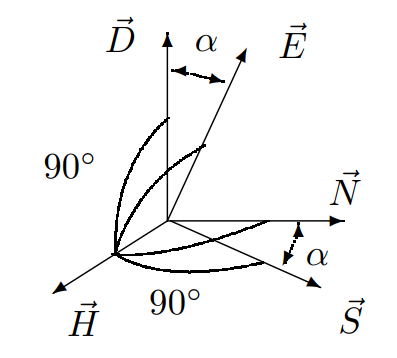
\includegraphics[width=0.8\linewidth]{fig1}
	\caption{Экспериментальная установка. (1) -- компьютер для сбора данных, (2) -- АЦП}
	\label{graph1:comp}
\end{figure}

\begin{figure}[h!]
	\centering
	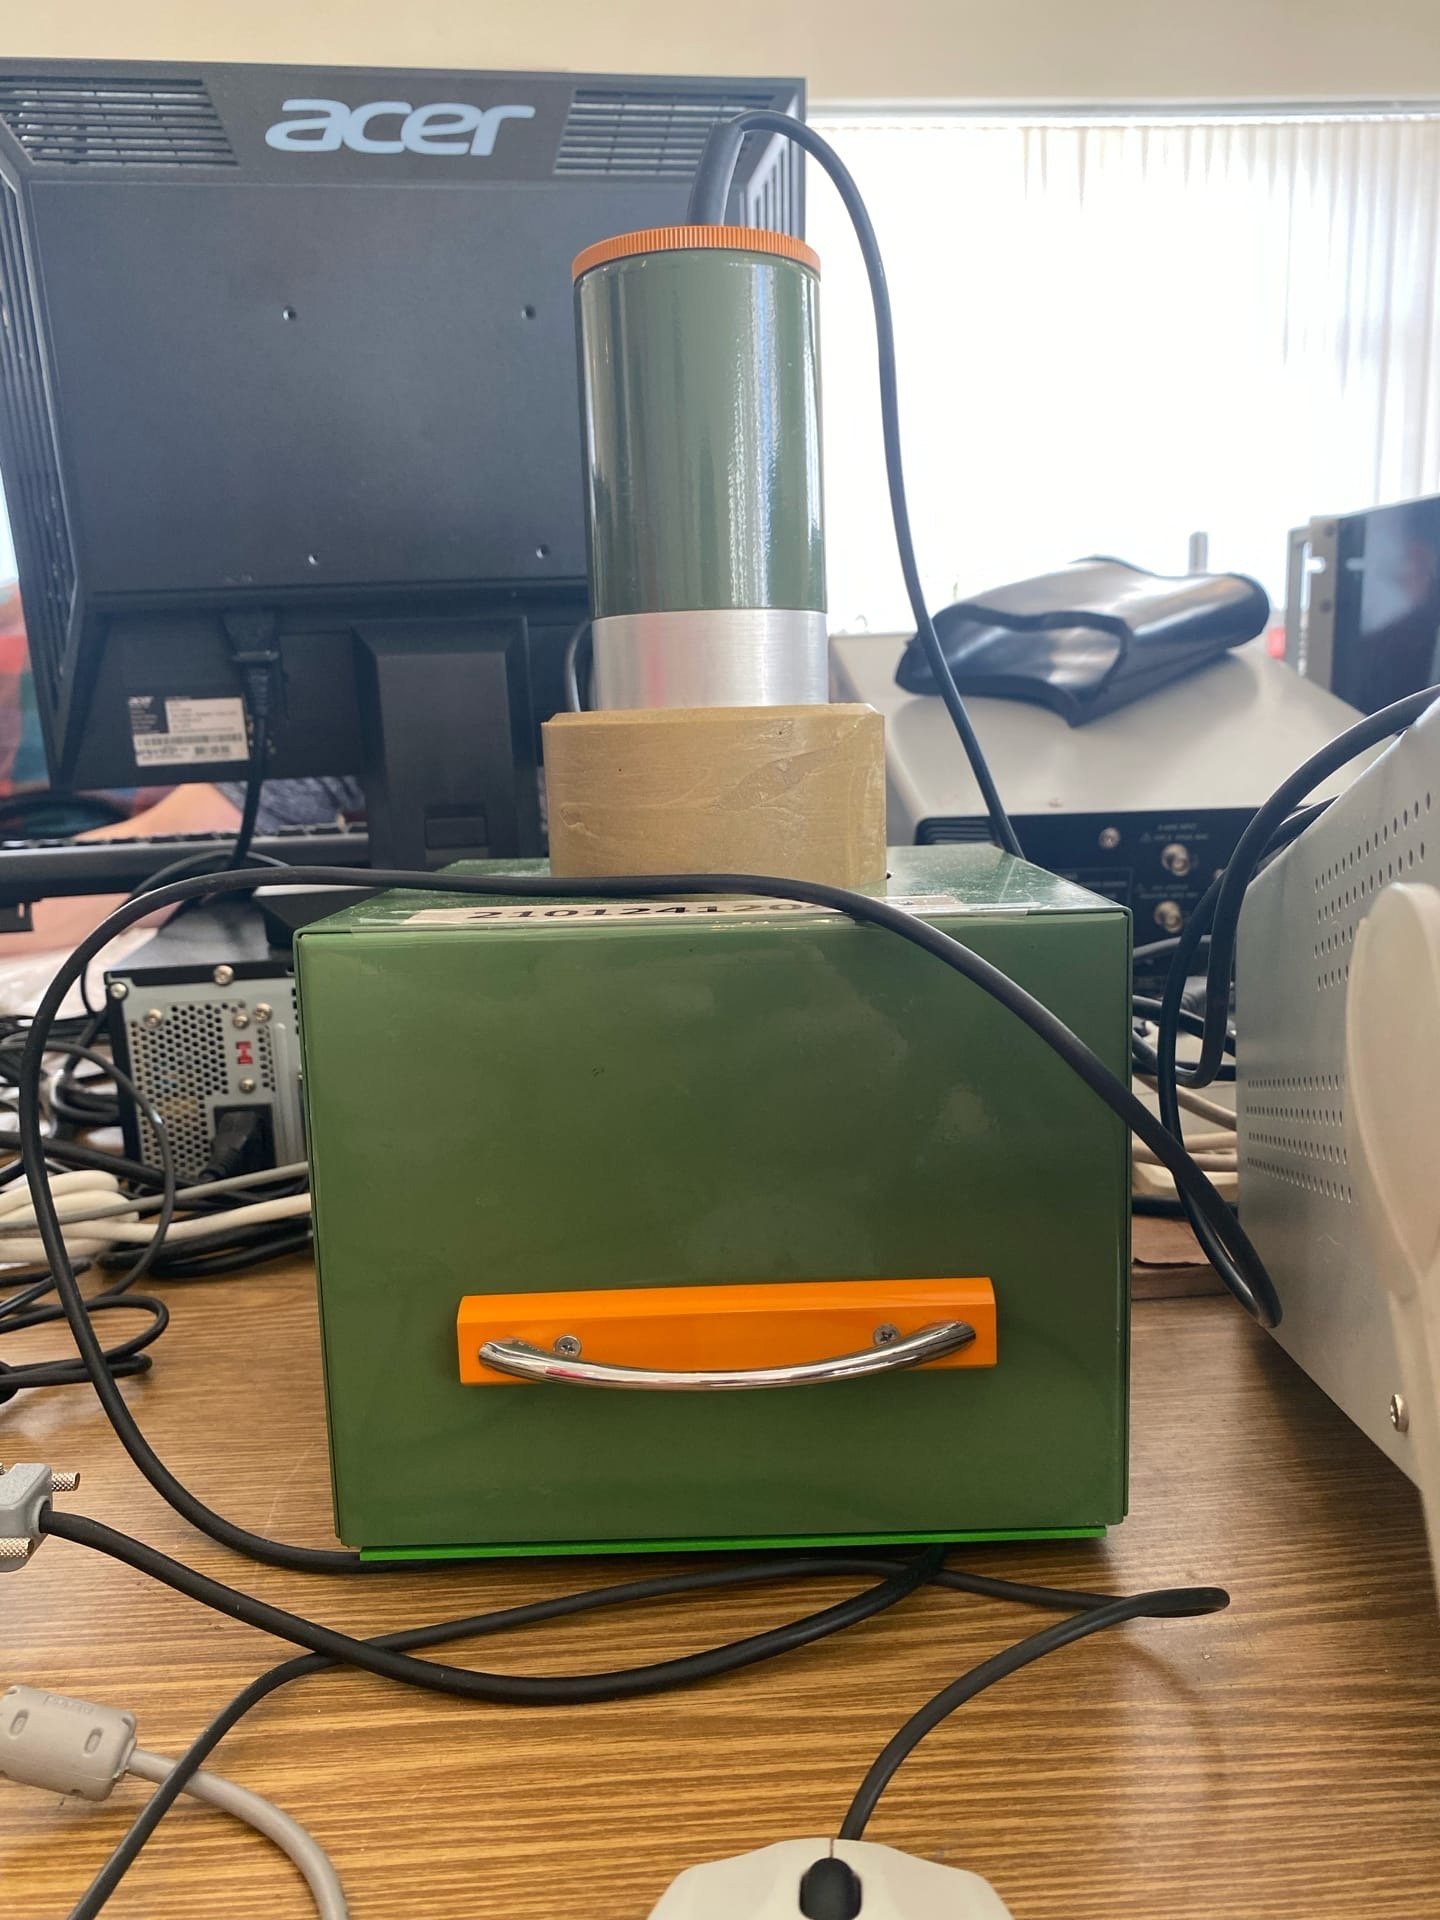
\includegraphics[width=0.8\linewidth]{fig2}
	\caption{Экспериментальная установка. Блок, включающий в себя ФЭУ, сцинтиллятор и отсек для образцов)}
	\label{fig2:FEU}
\end{figure}

\section*{Ход работы}
Перед измерениями спектров измерим фон в течение 600 секунд 
(представлен на  \\ Рис. (\ref{graph1:background})).

\newpage 

\begin{figure}[h]
	\centering
	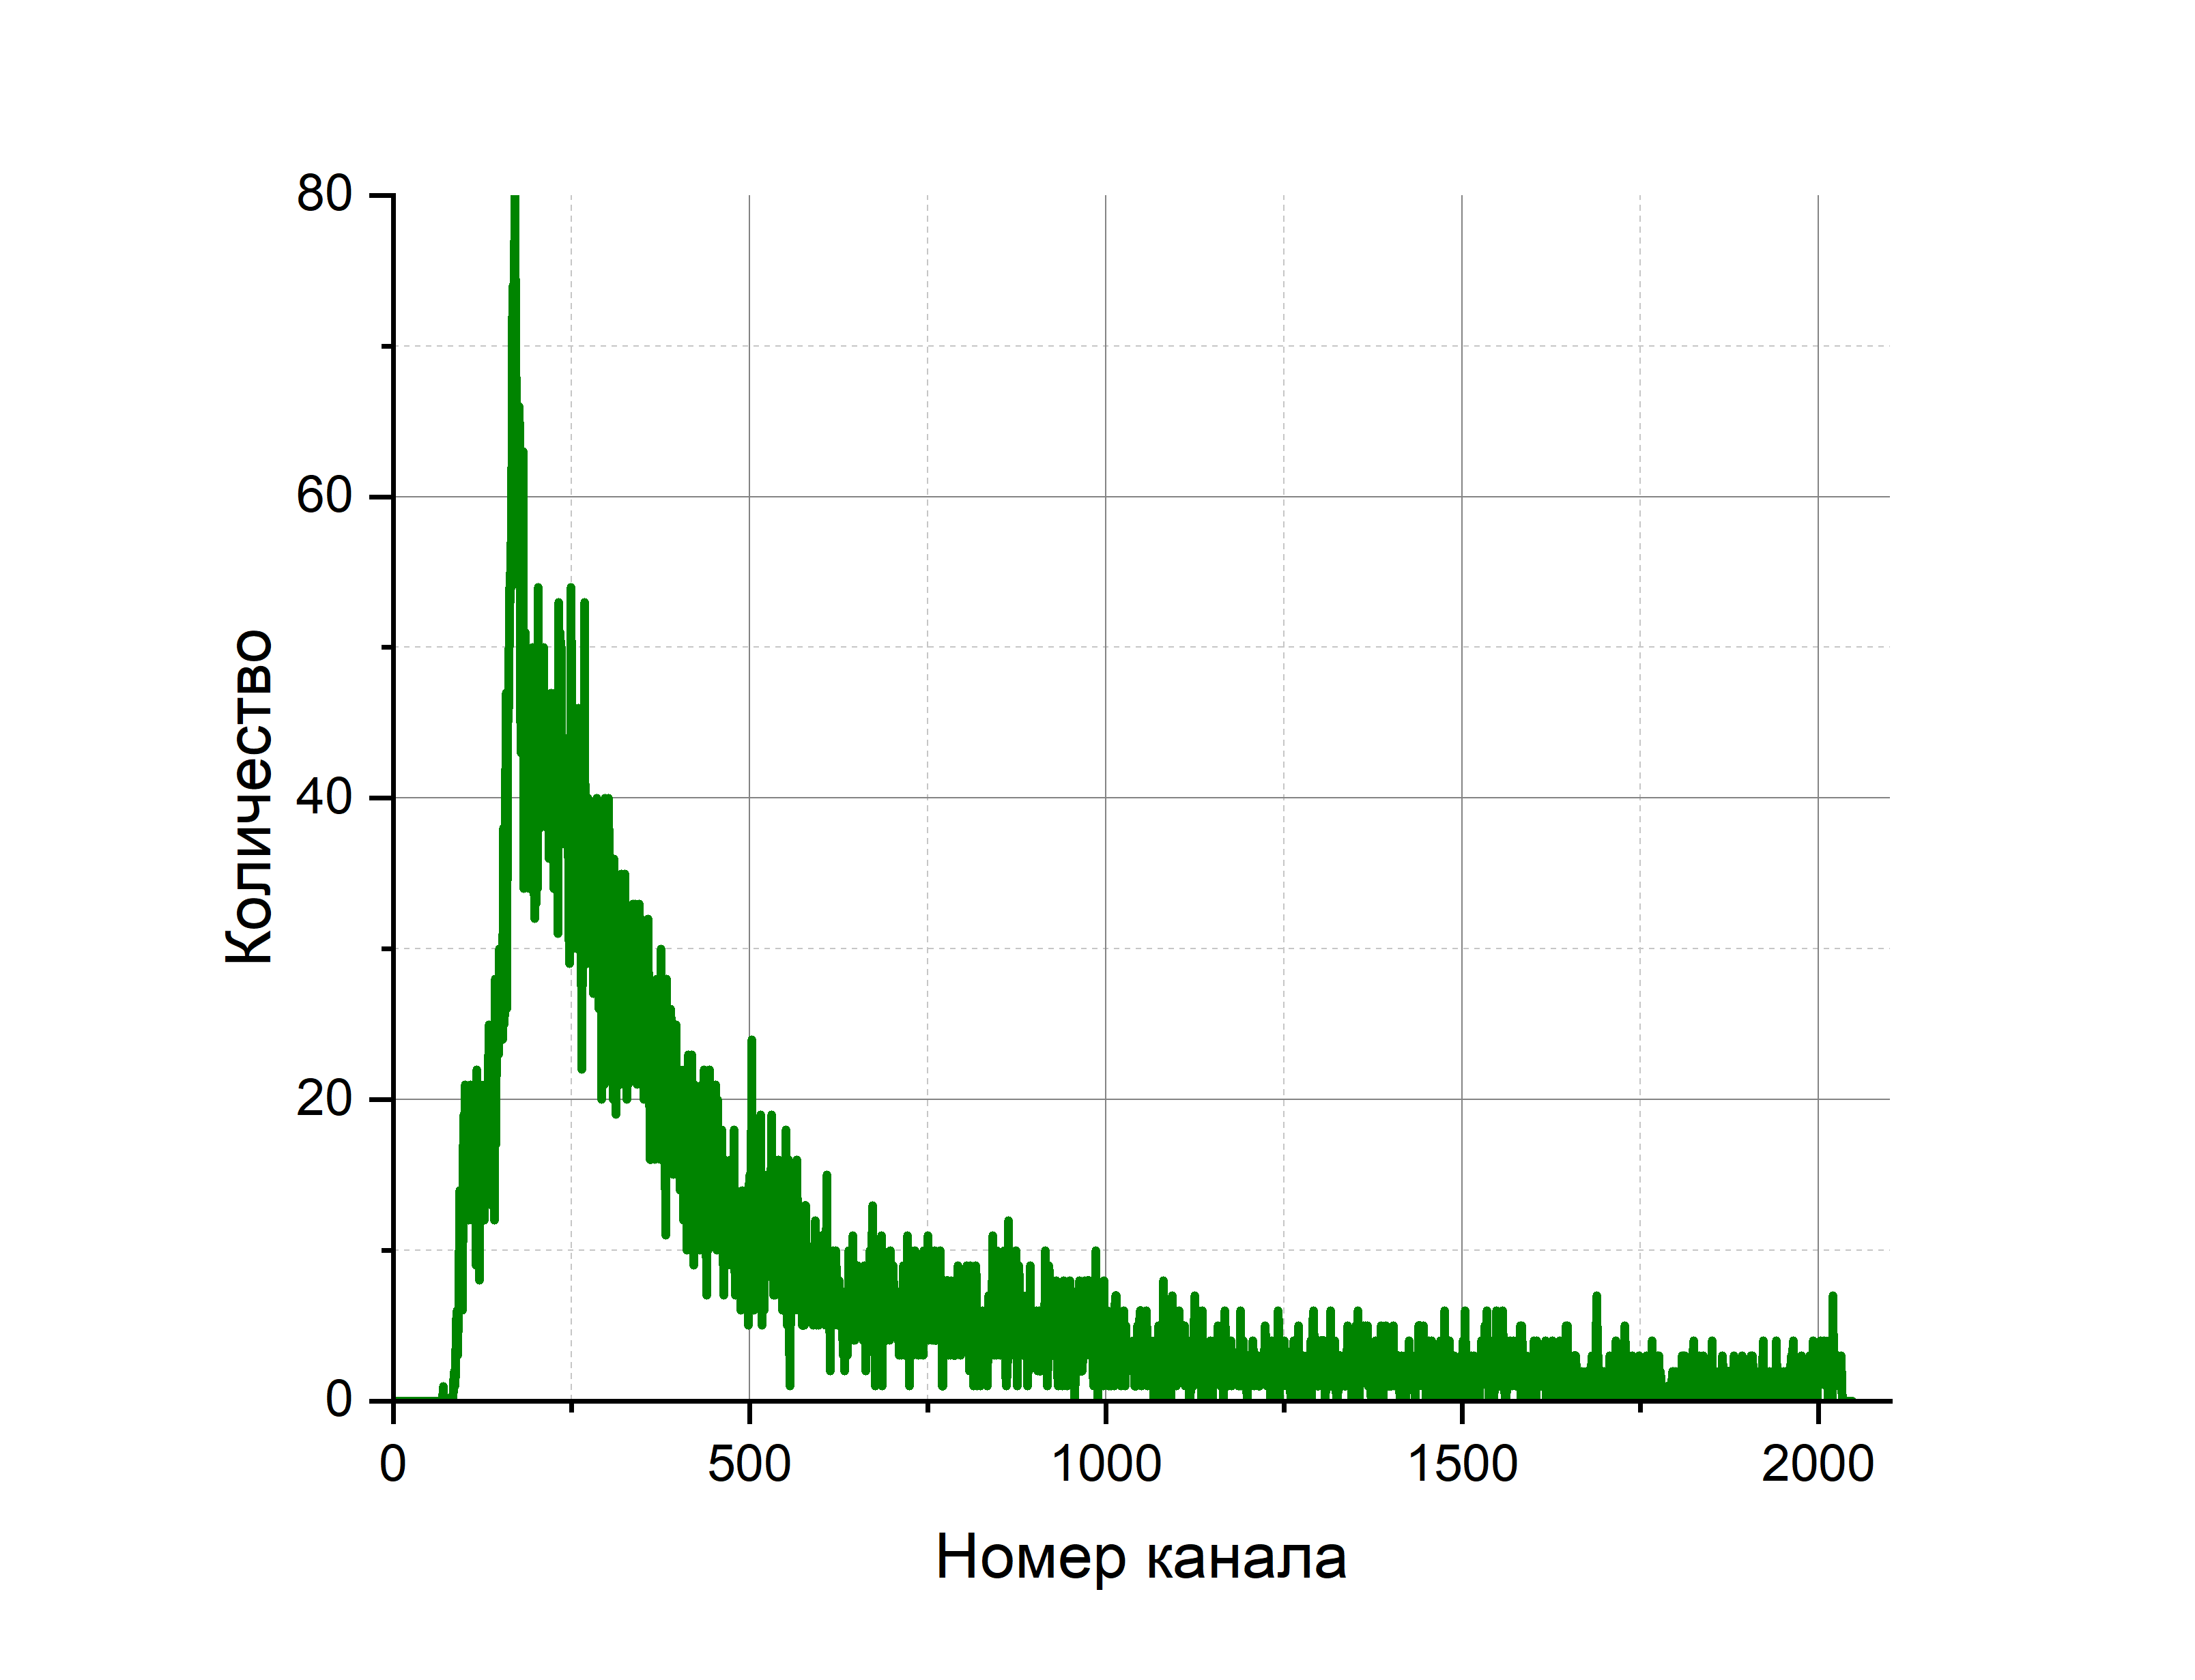
\includegraphics[width=0.8\linewidth]{graph8}
	\caption{Спектр для фона (без образца)}
	\label{graph1:background}
\end{figure} 
 
Далее проведем измерения спектров в течение 600 секунд для образцов:

\begin{itemize}
\item $^{60}Co$
\item $^{137}Cs$
\item $^{152}Eu$
\item $^{241}Am$
\item $^{22}Na$
\end{itemize}
  
 
Спектры данных образцов (с исключенным фоном) представлены на Рисунках (\ref{graph2:Co}) - (\ref{graph6:Na}) 
 
\newpage 
 
\begin{figure}[h!]
	\centering
	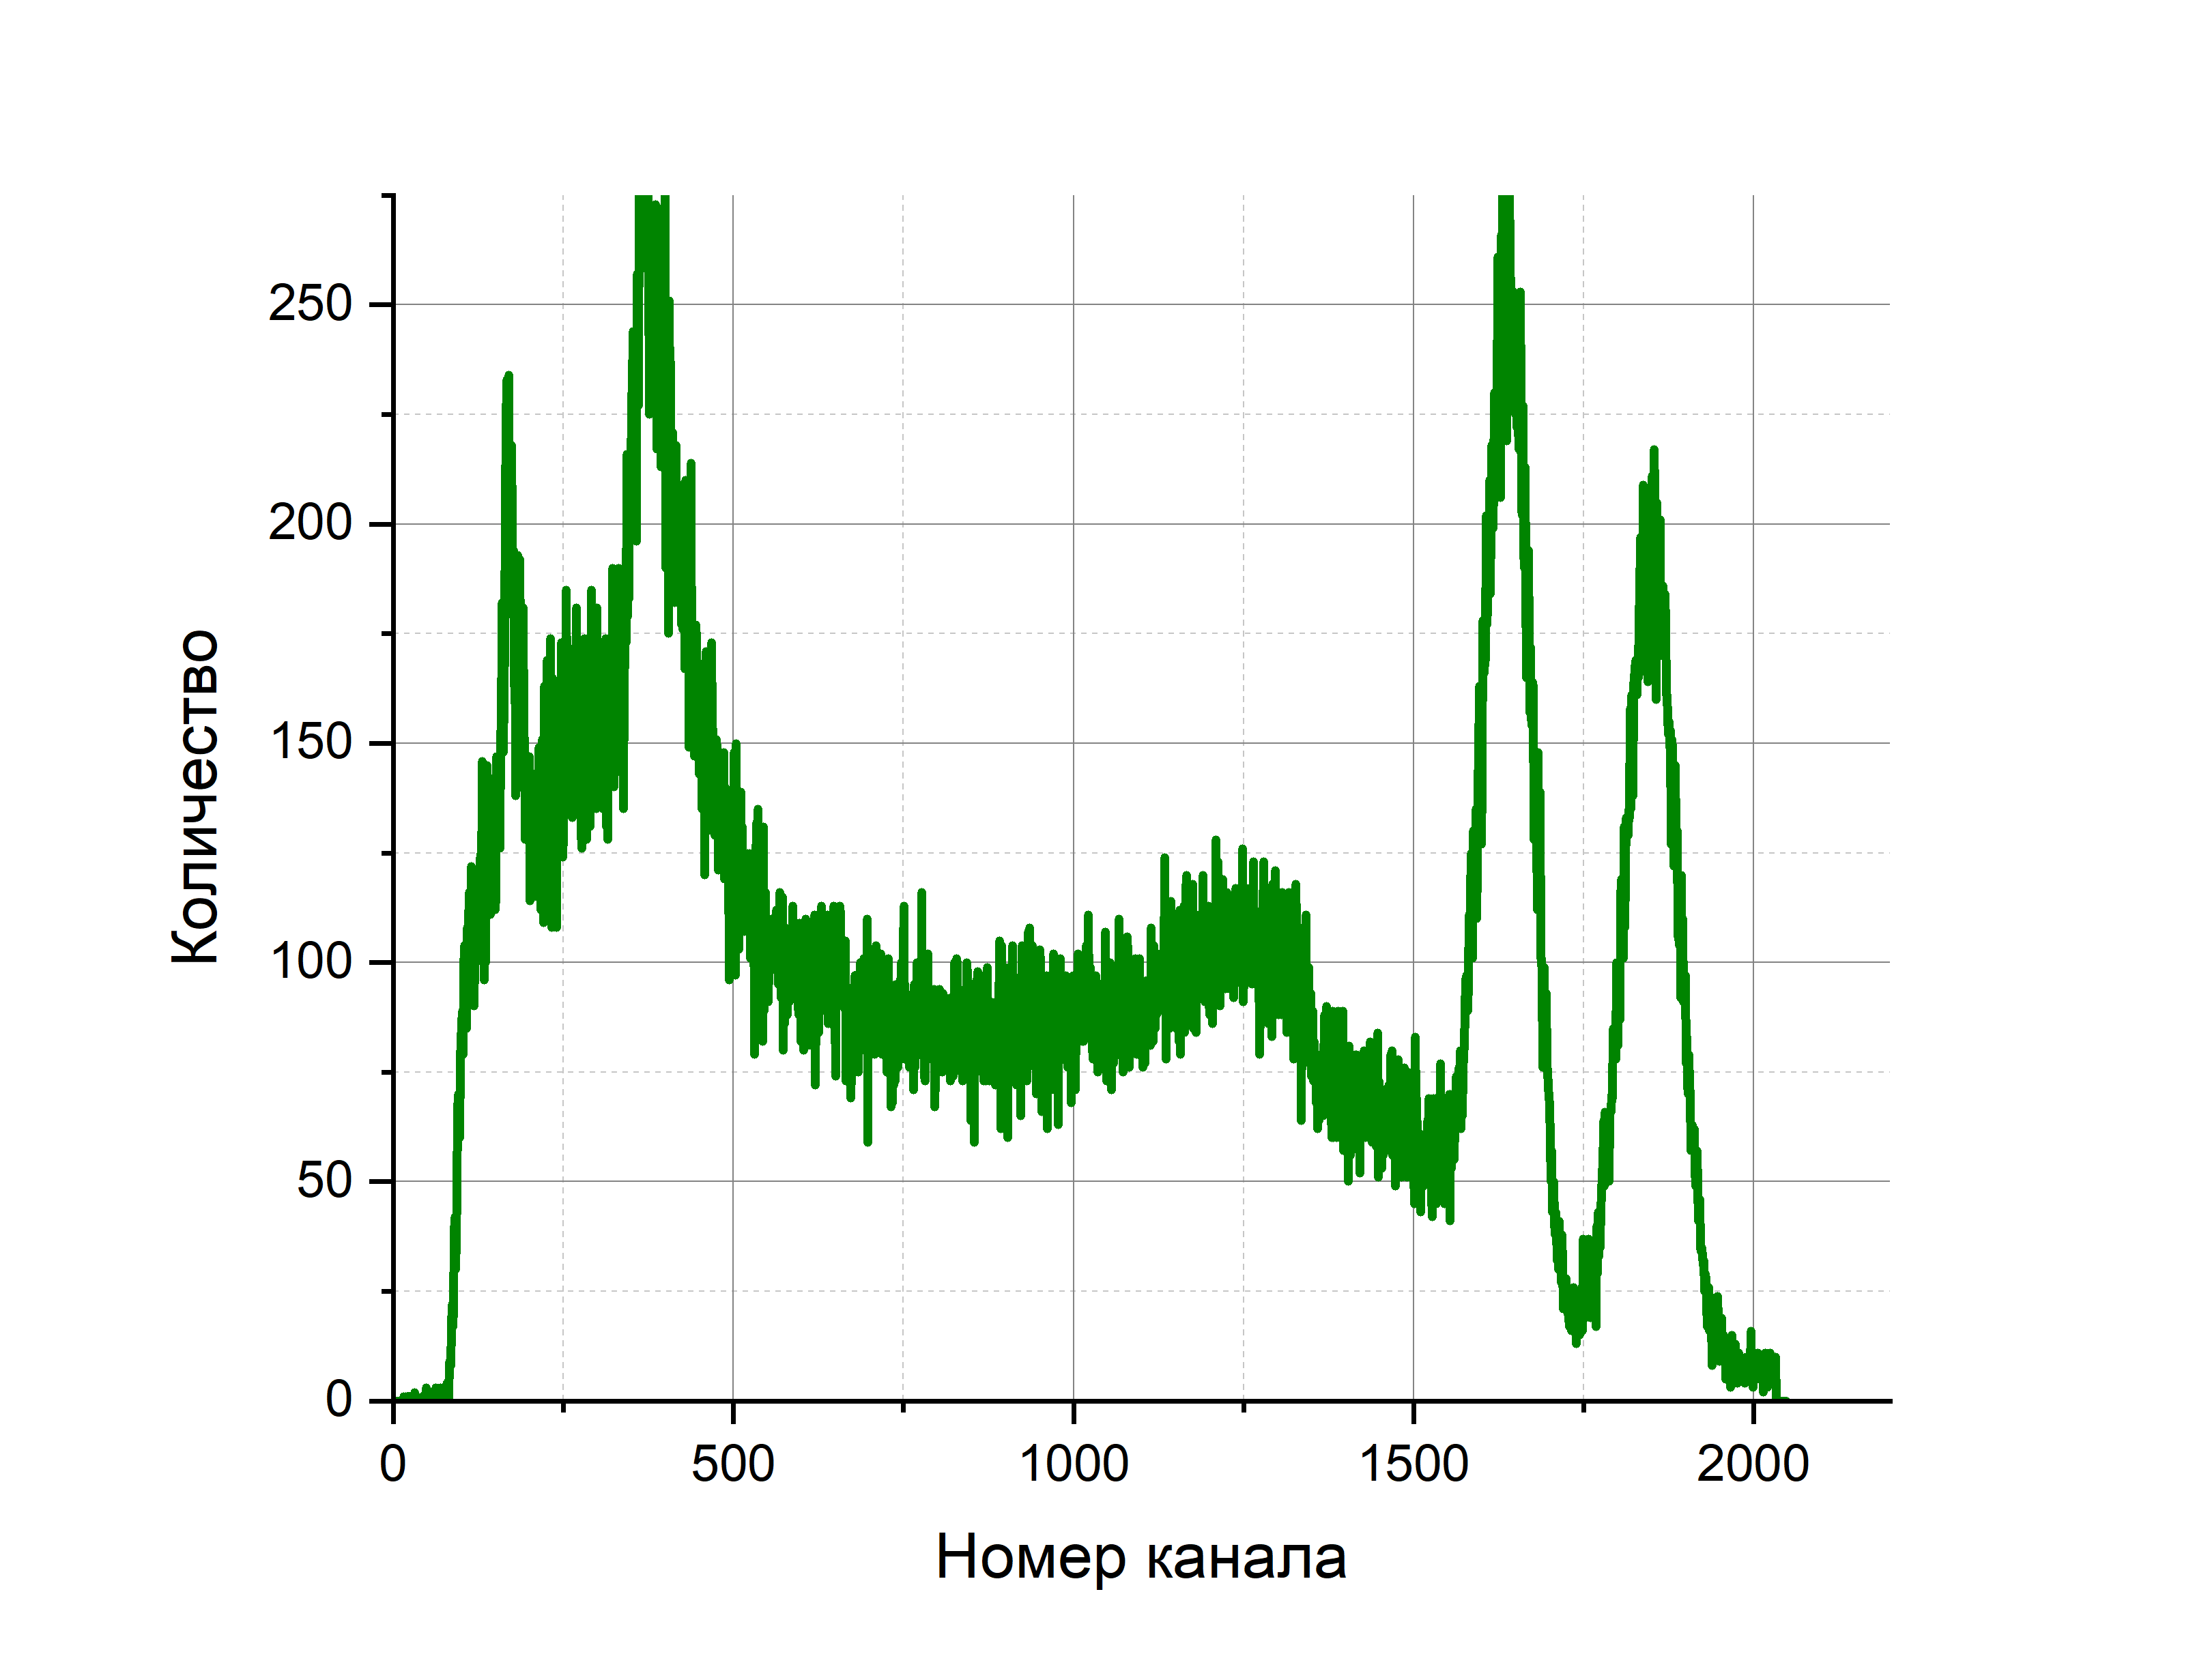
\includegraphics[width=0.8\linewidth]{graph3}
	\caption{Спектр для $^{60}Co$}
	\label{graph2:Co}
\end{figure}

\begin{figure}[h!]
	\centering
	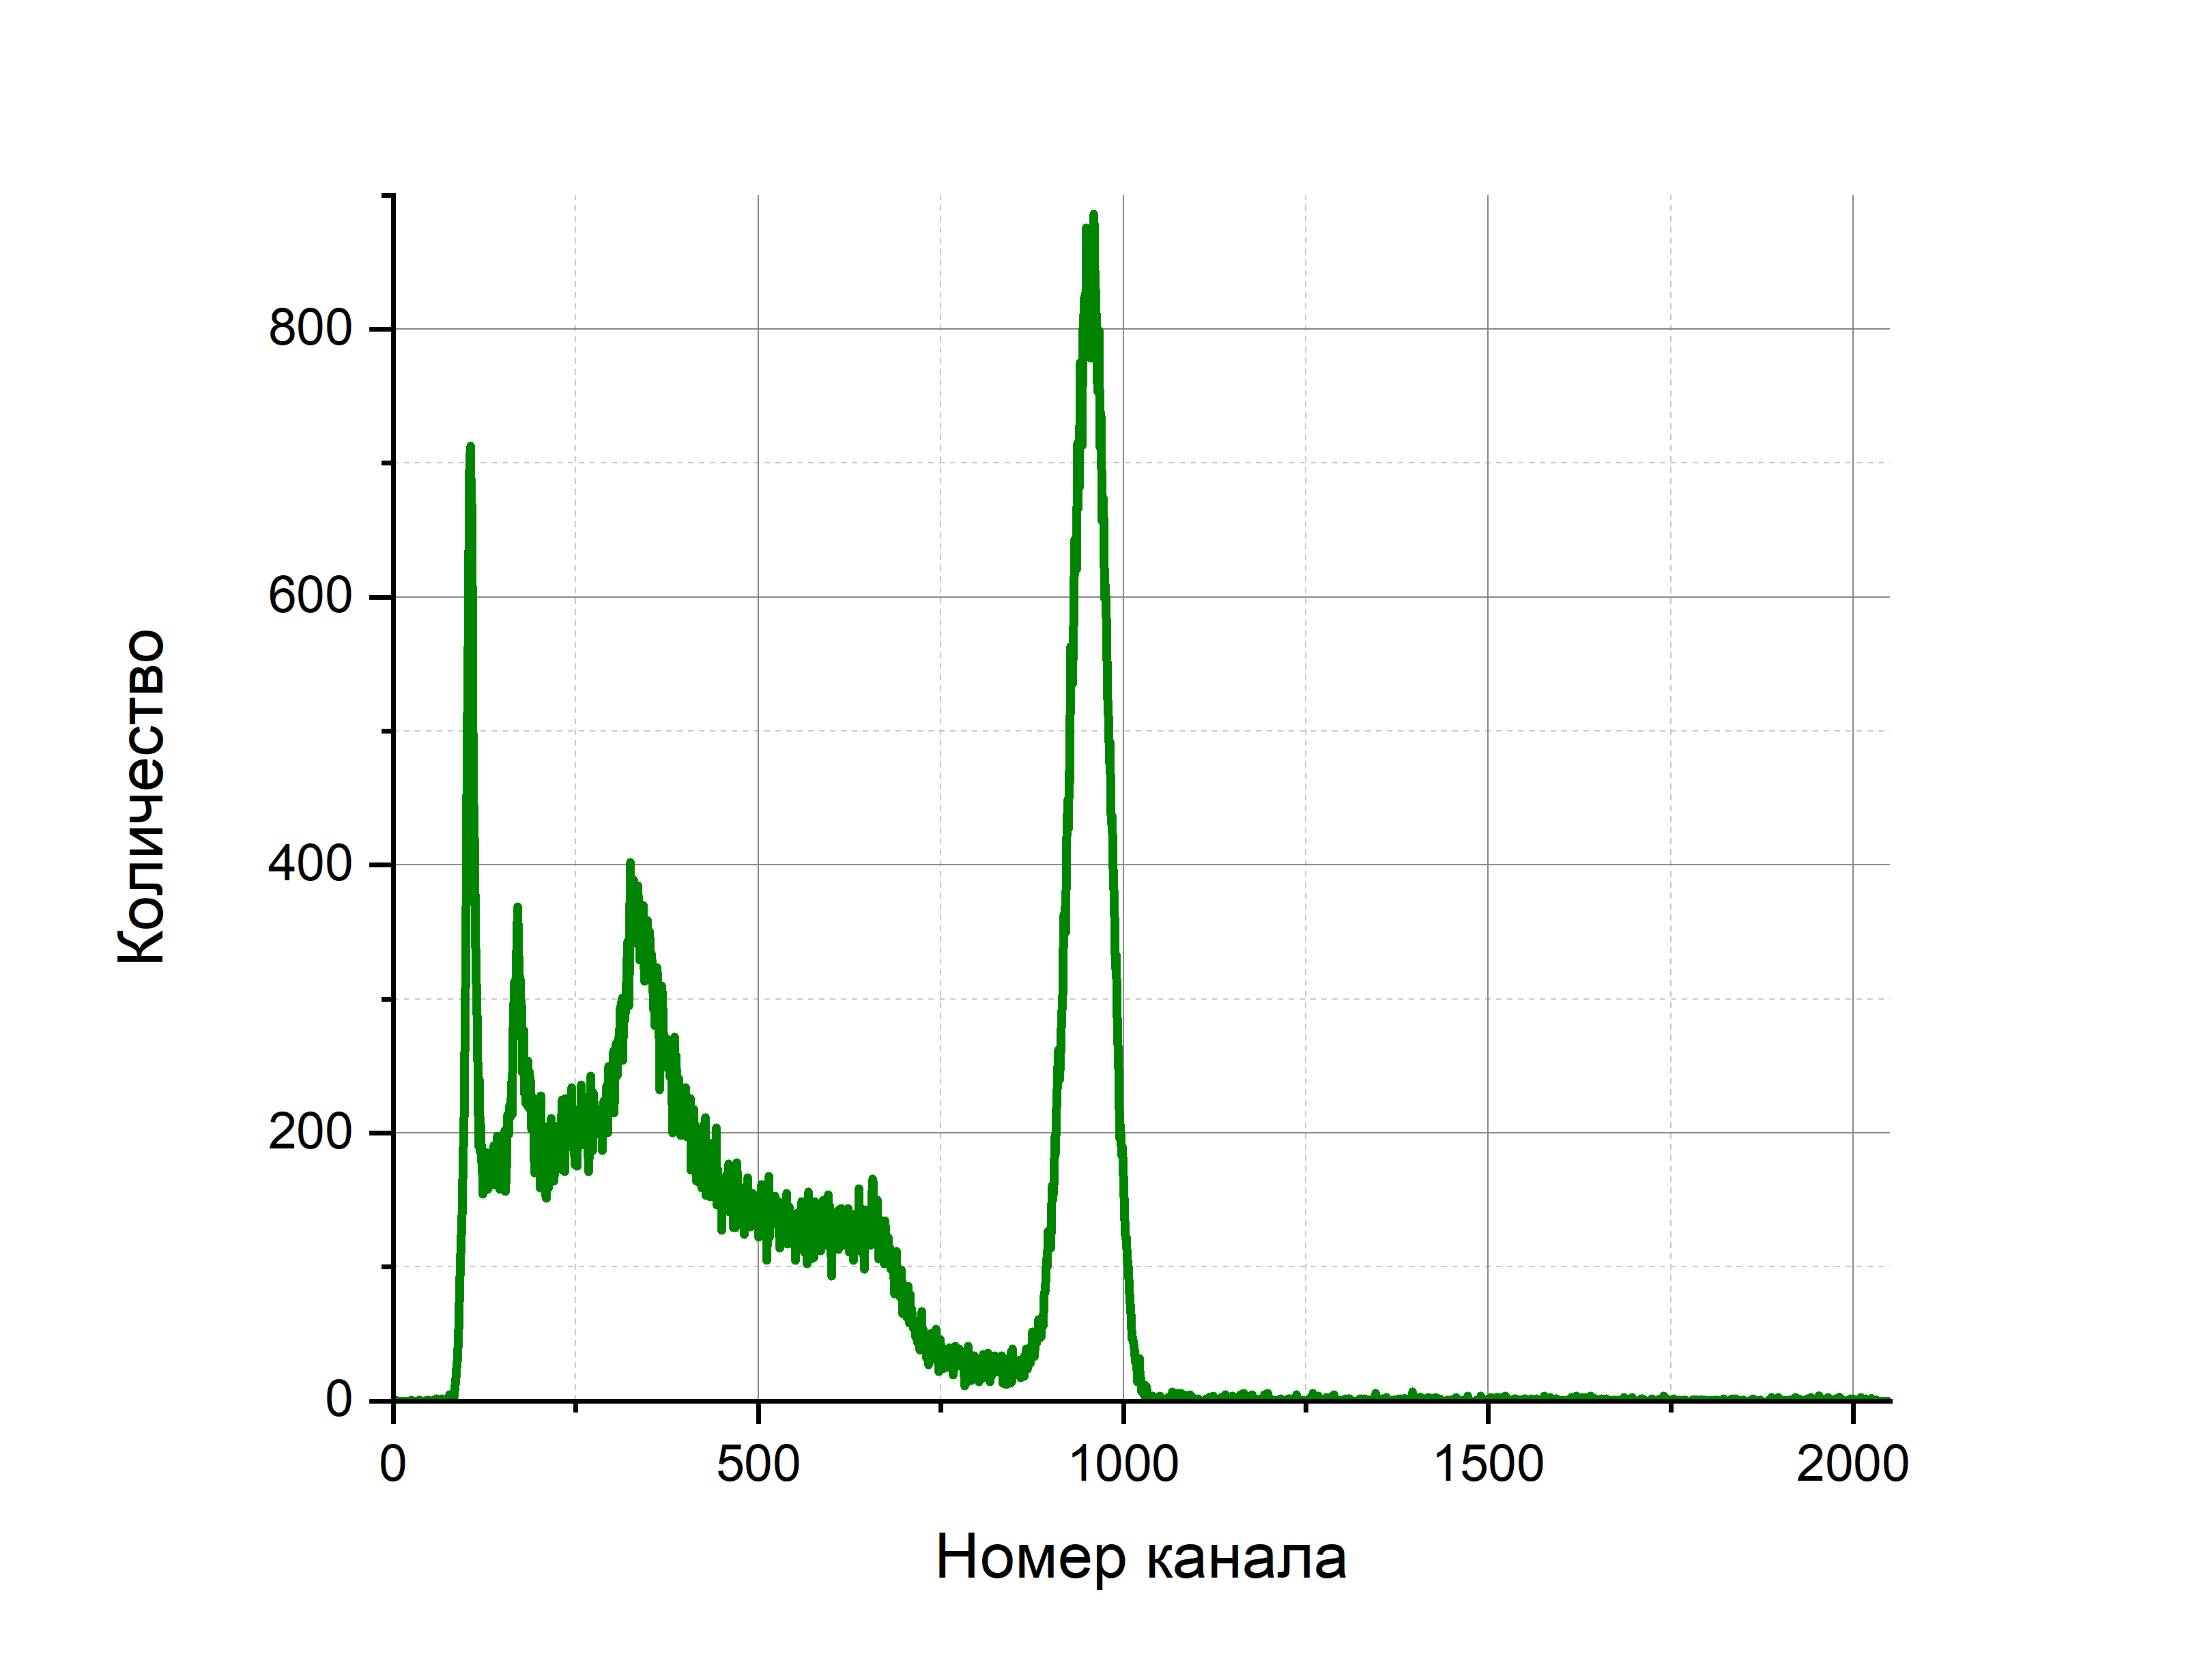
\includegraphics[width=0.8\linewidth]{graph4}
	\caption{Спектр для  $^{137}Cs$}
	\label{graph3:Cs}
\end{figure}

\newpage

\begin{figure}[h!]
	\centering
	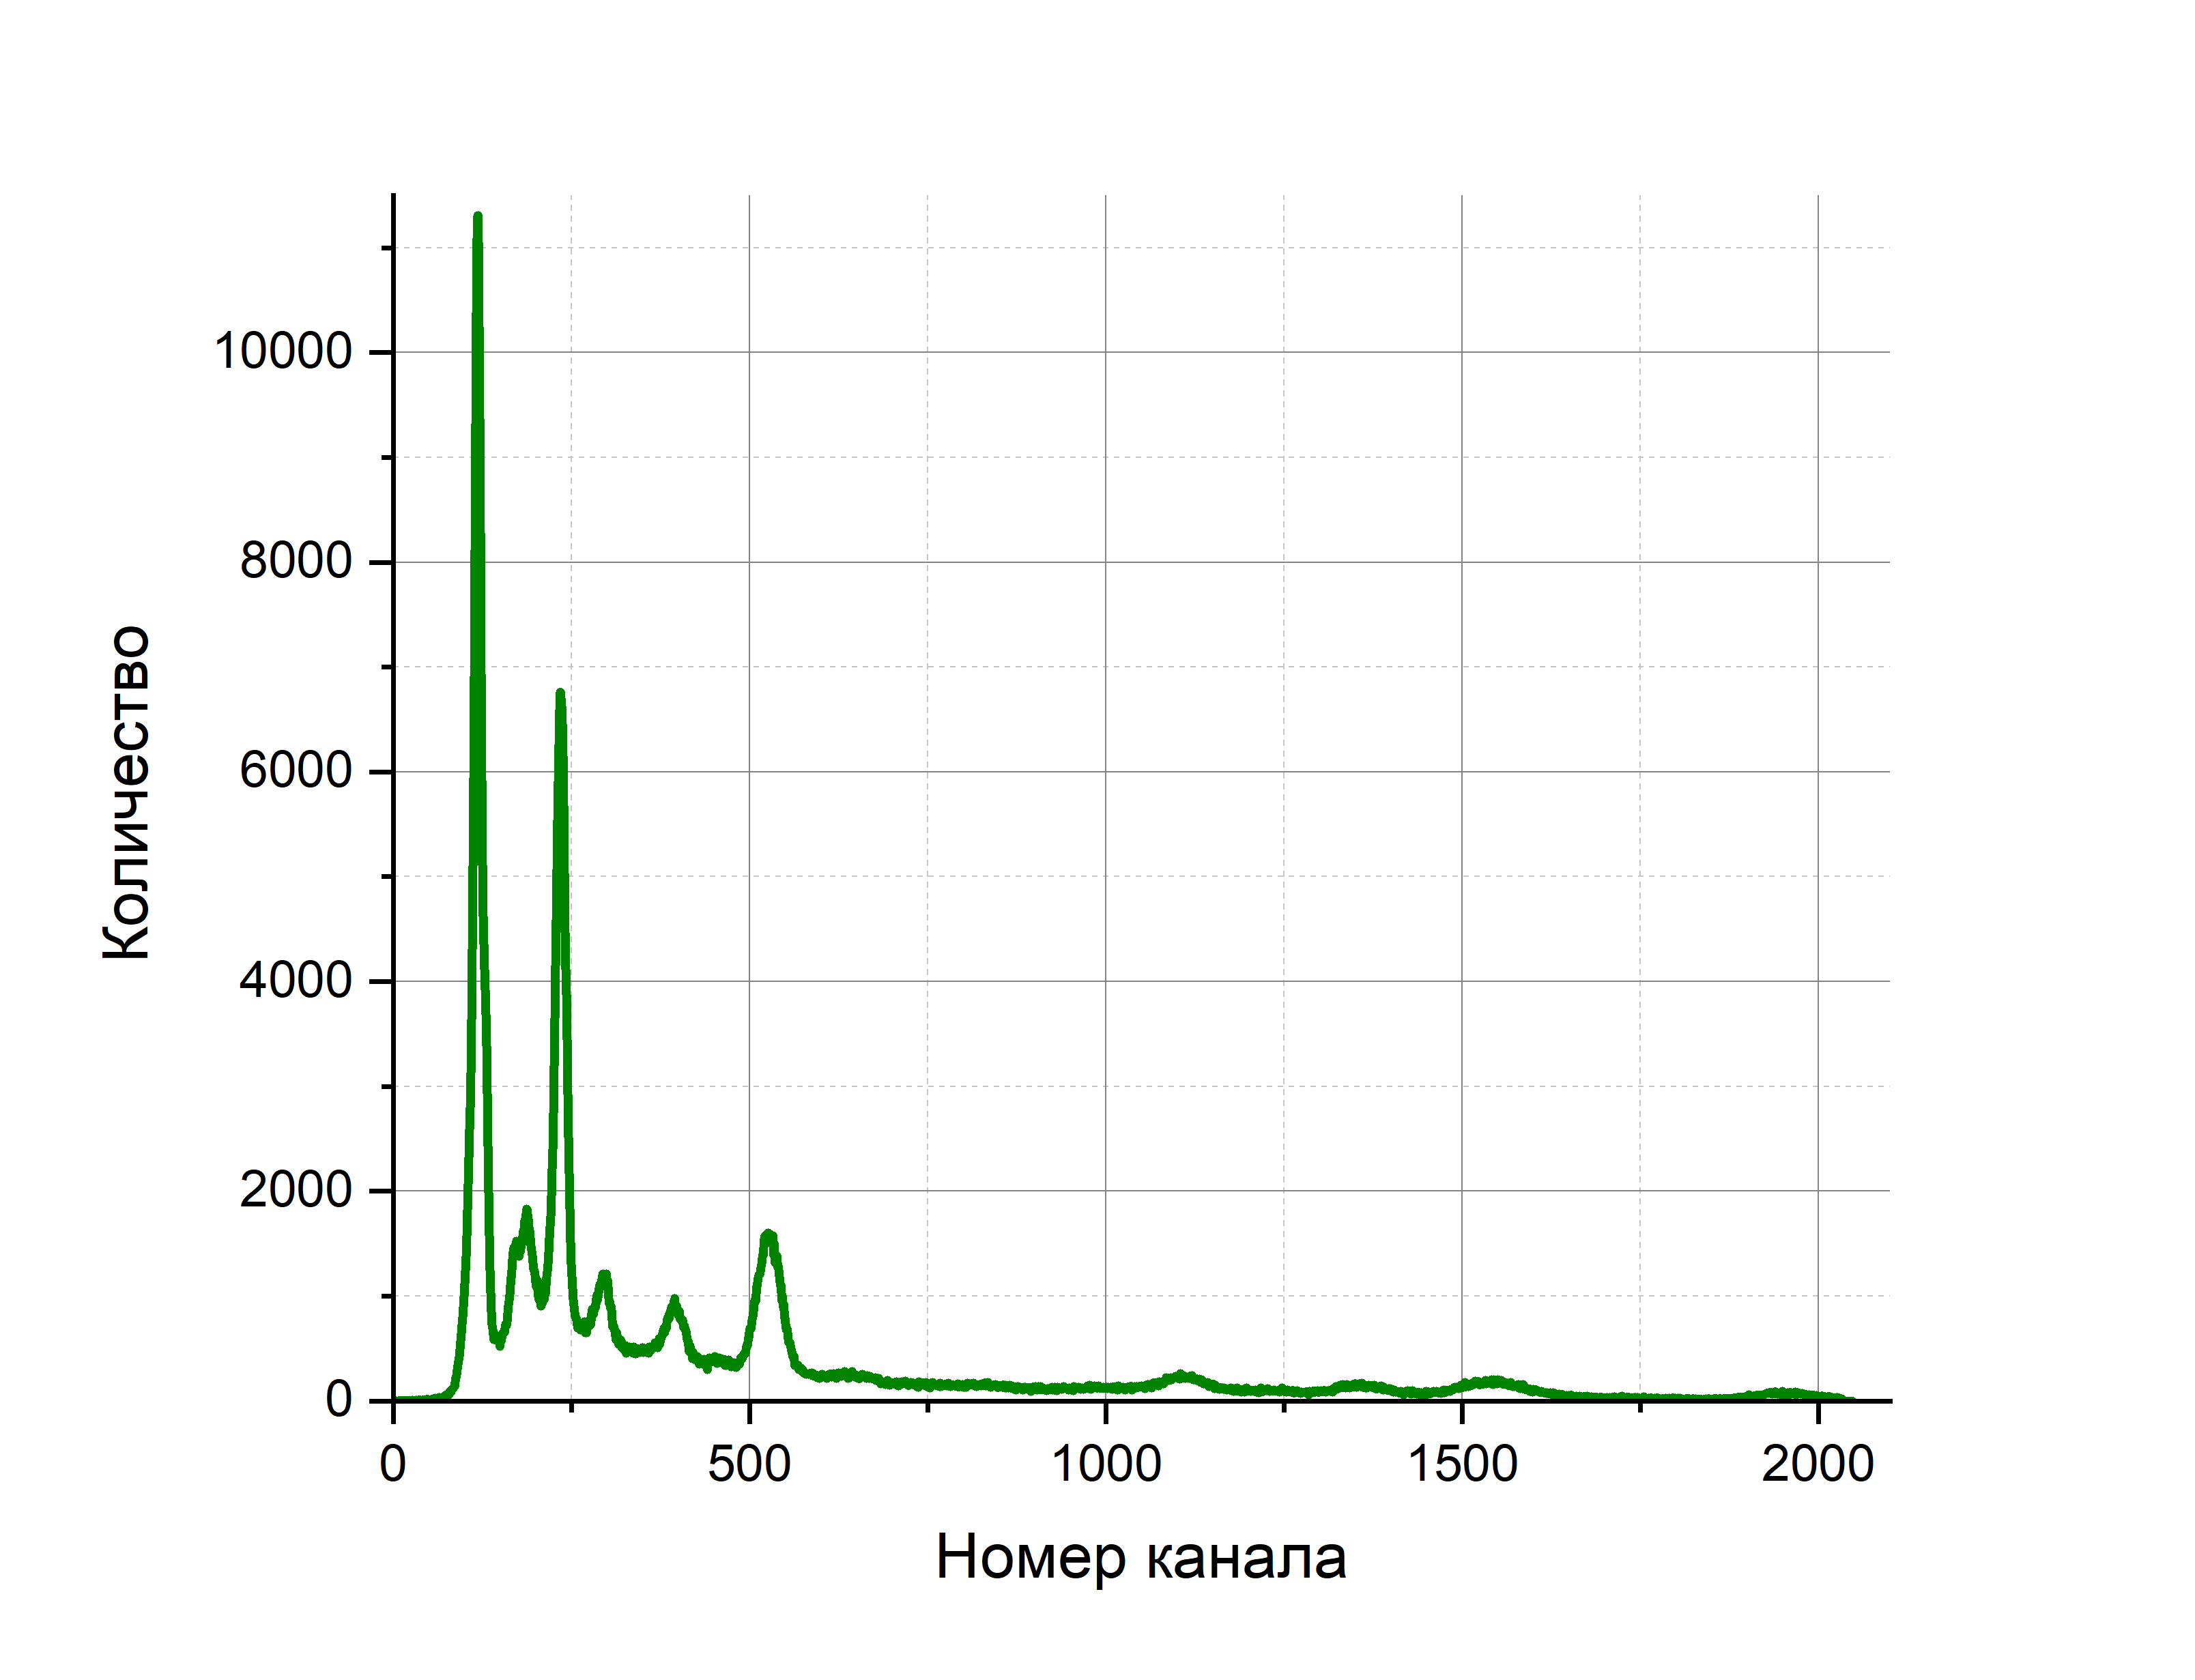
\includegraphics[width=0.8\linewidth]{graph5}
	\caption{Спектр для $^{152}Eu$}
	\label{graph4:Eu}
\end{figure}

\begin{figure}[h!]
	\centering
	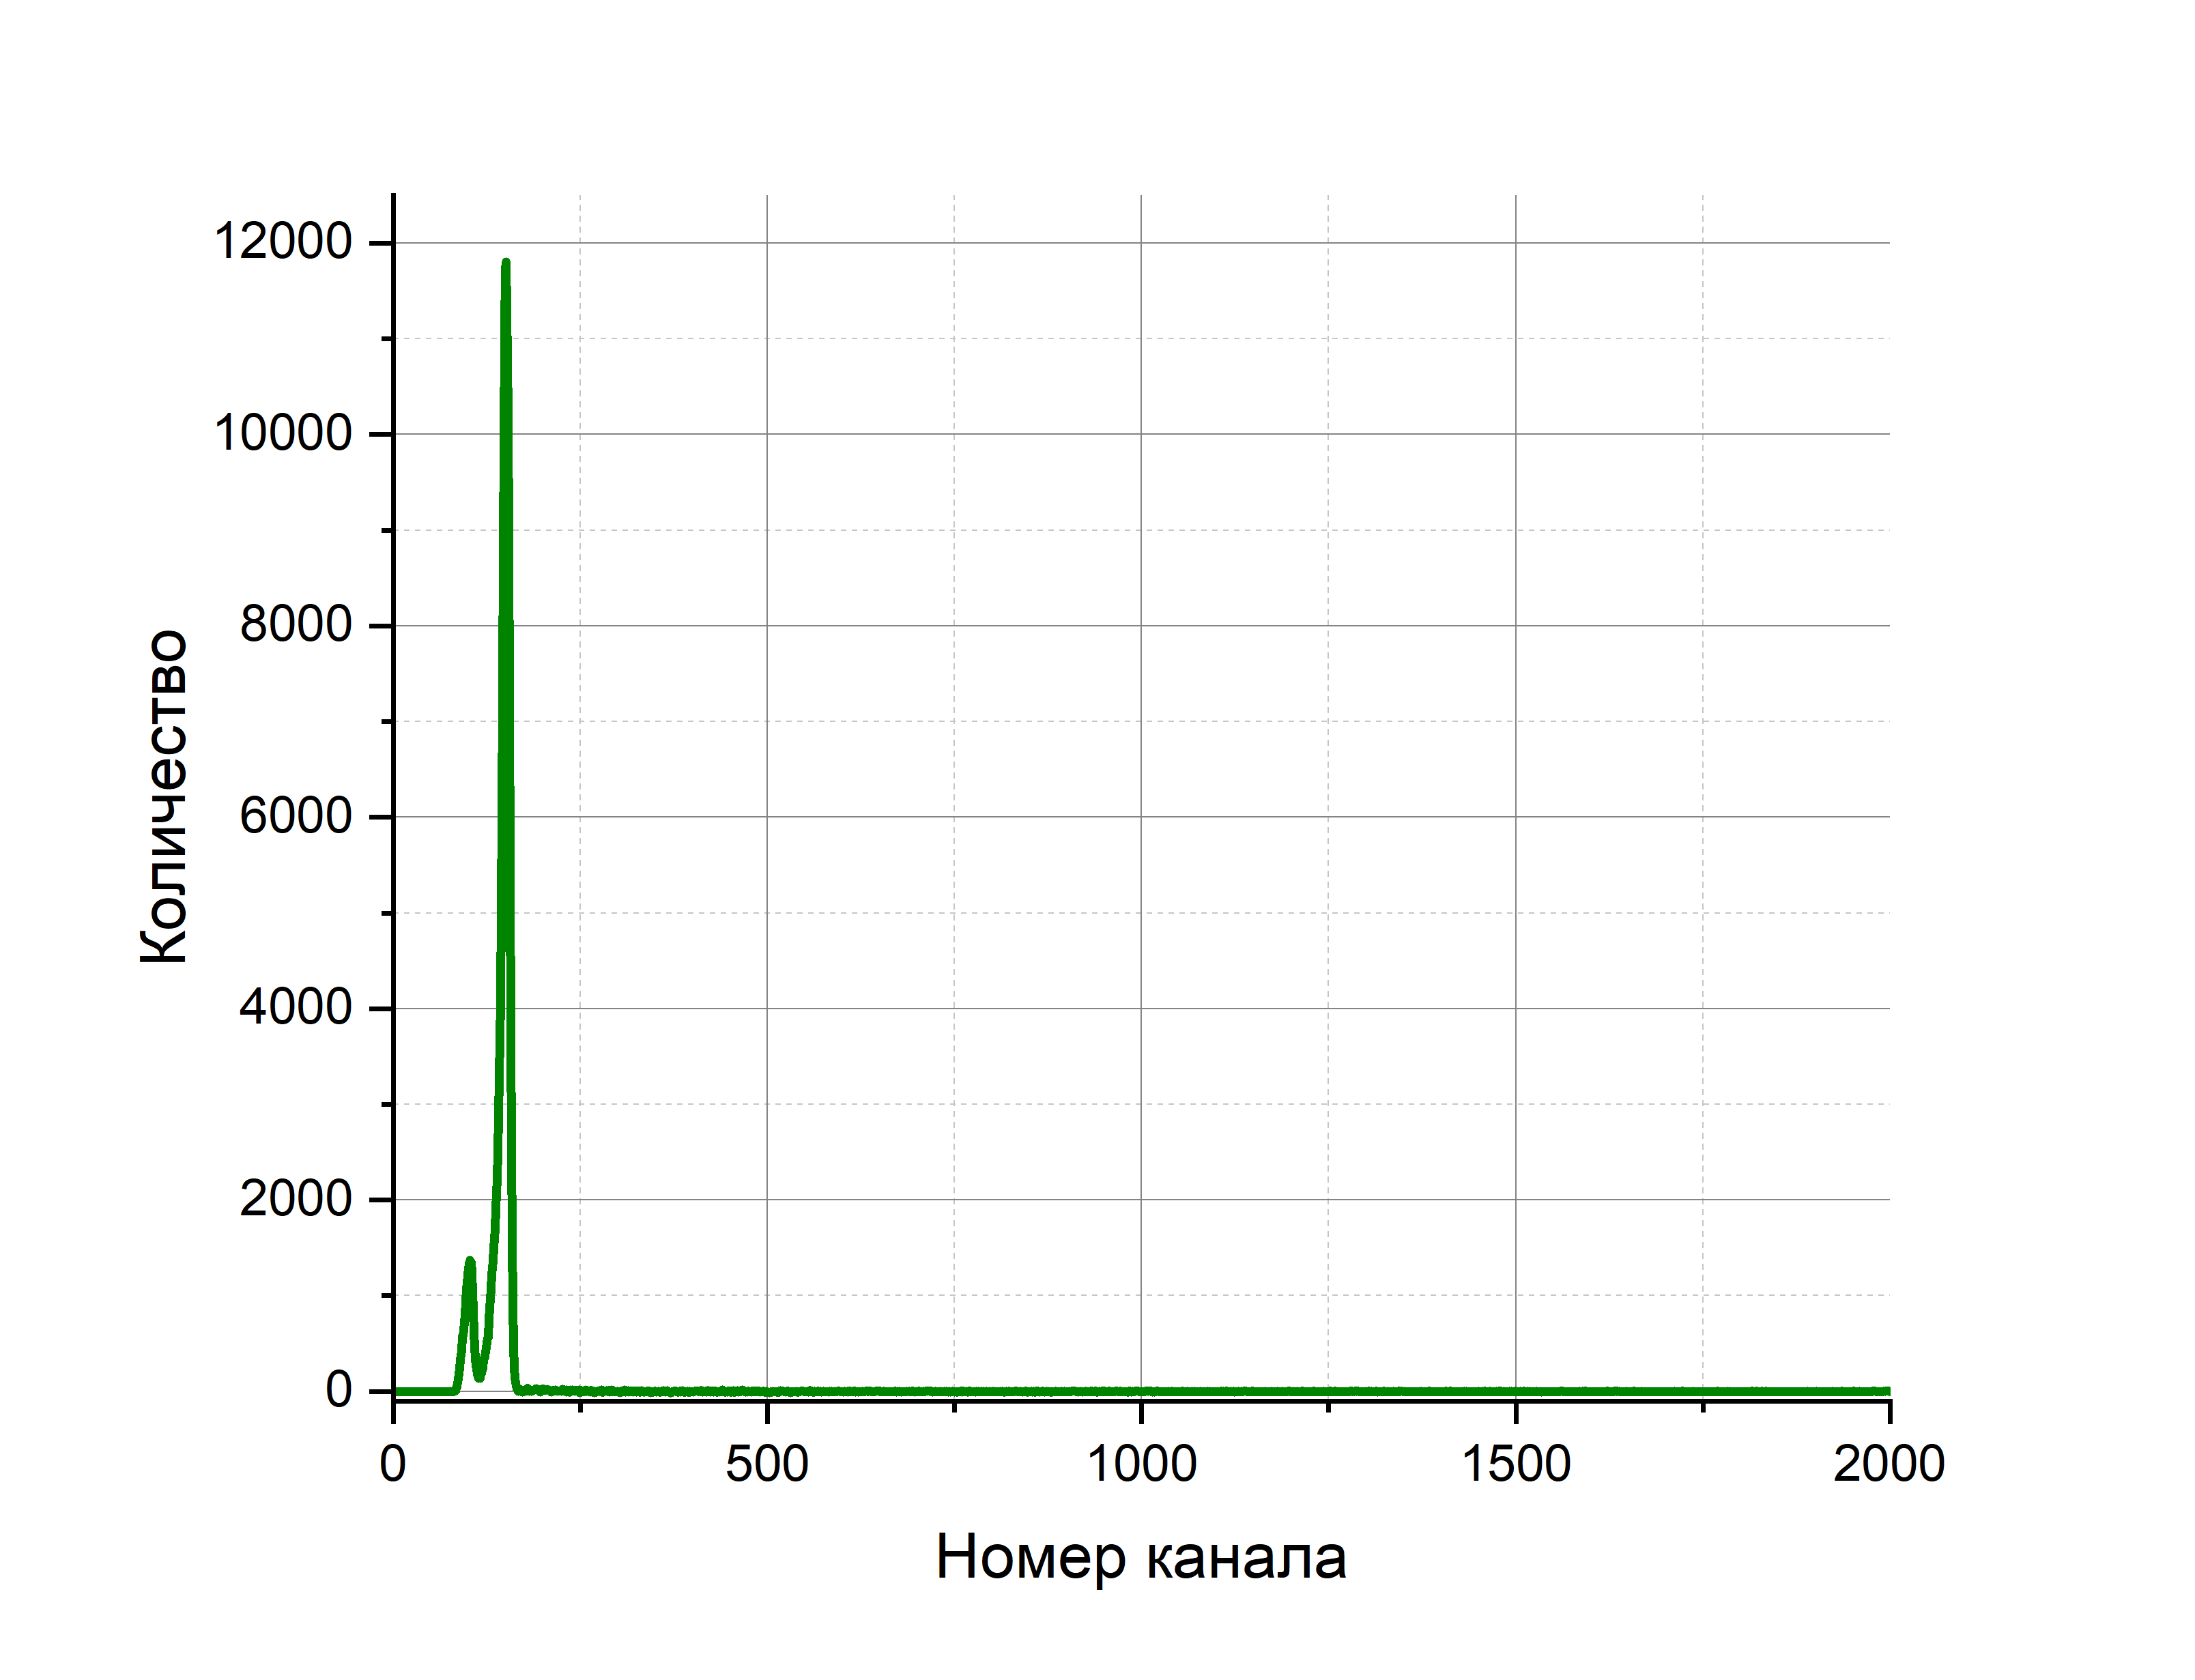
\includegraphics[width=0.8\linewidth]{graph6}
	\caption{Спектр для $^{241}Am$}
	\label{graph5:Am}
\end{figure}

\newpage

\begin{figure}[h!]
	\centering
	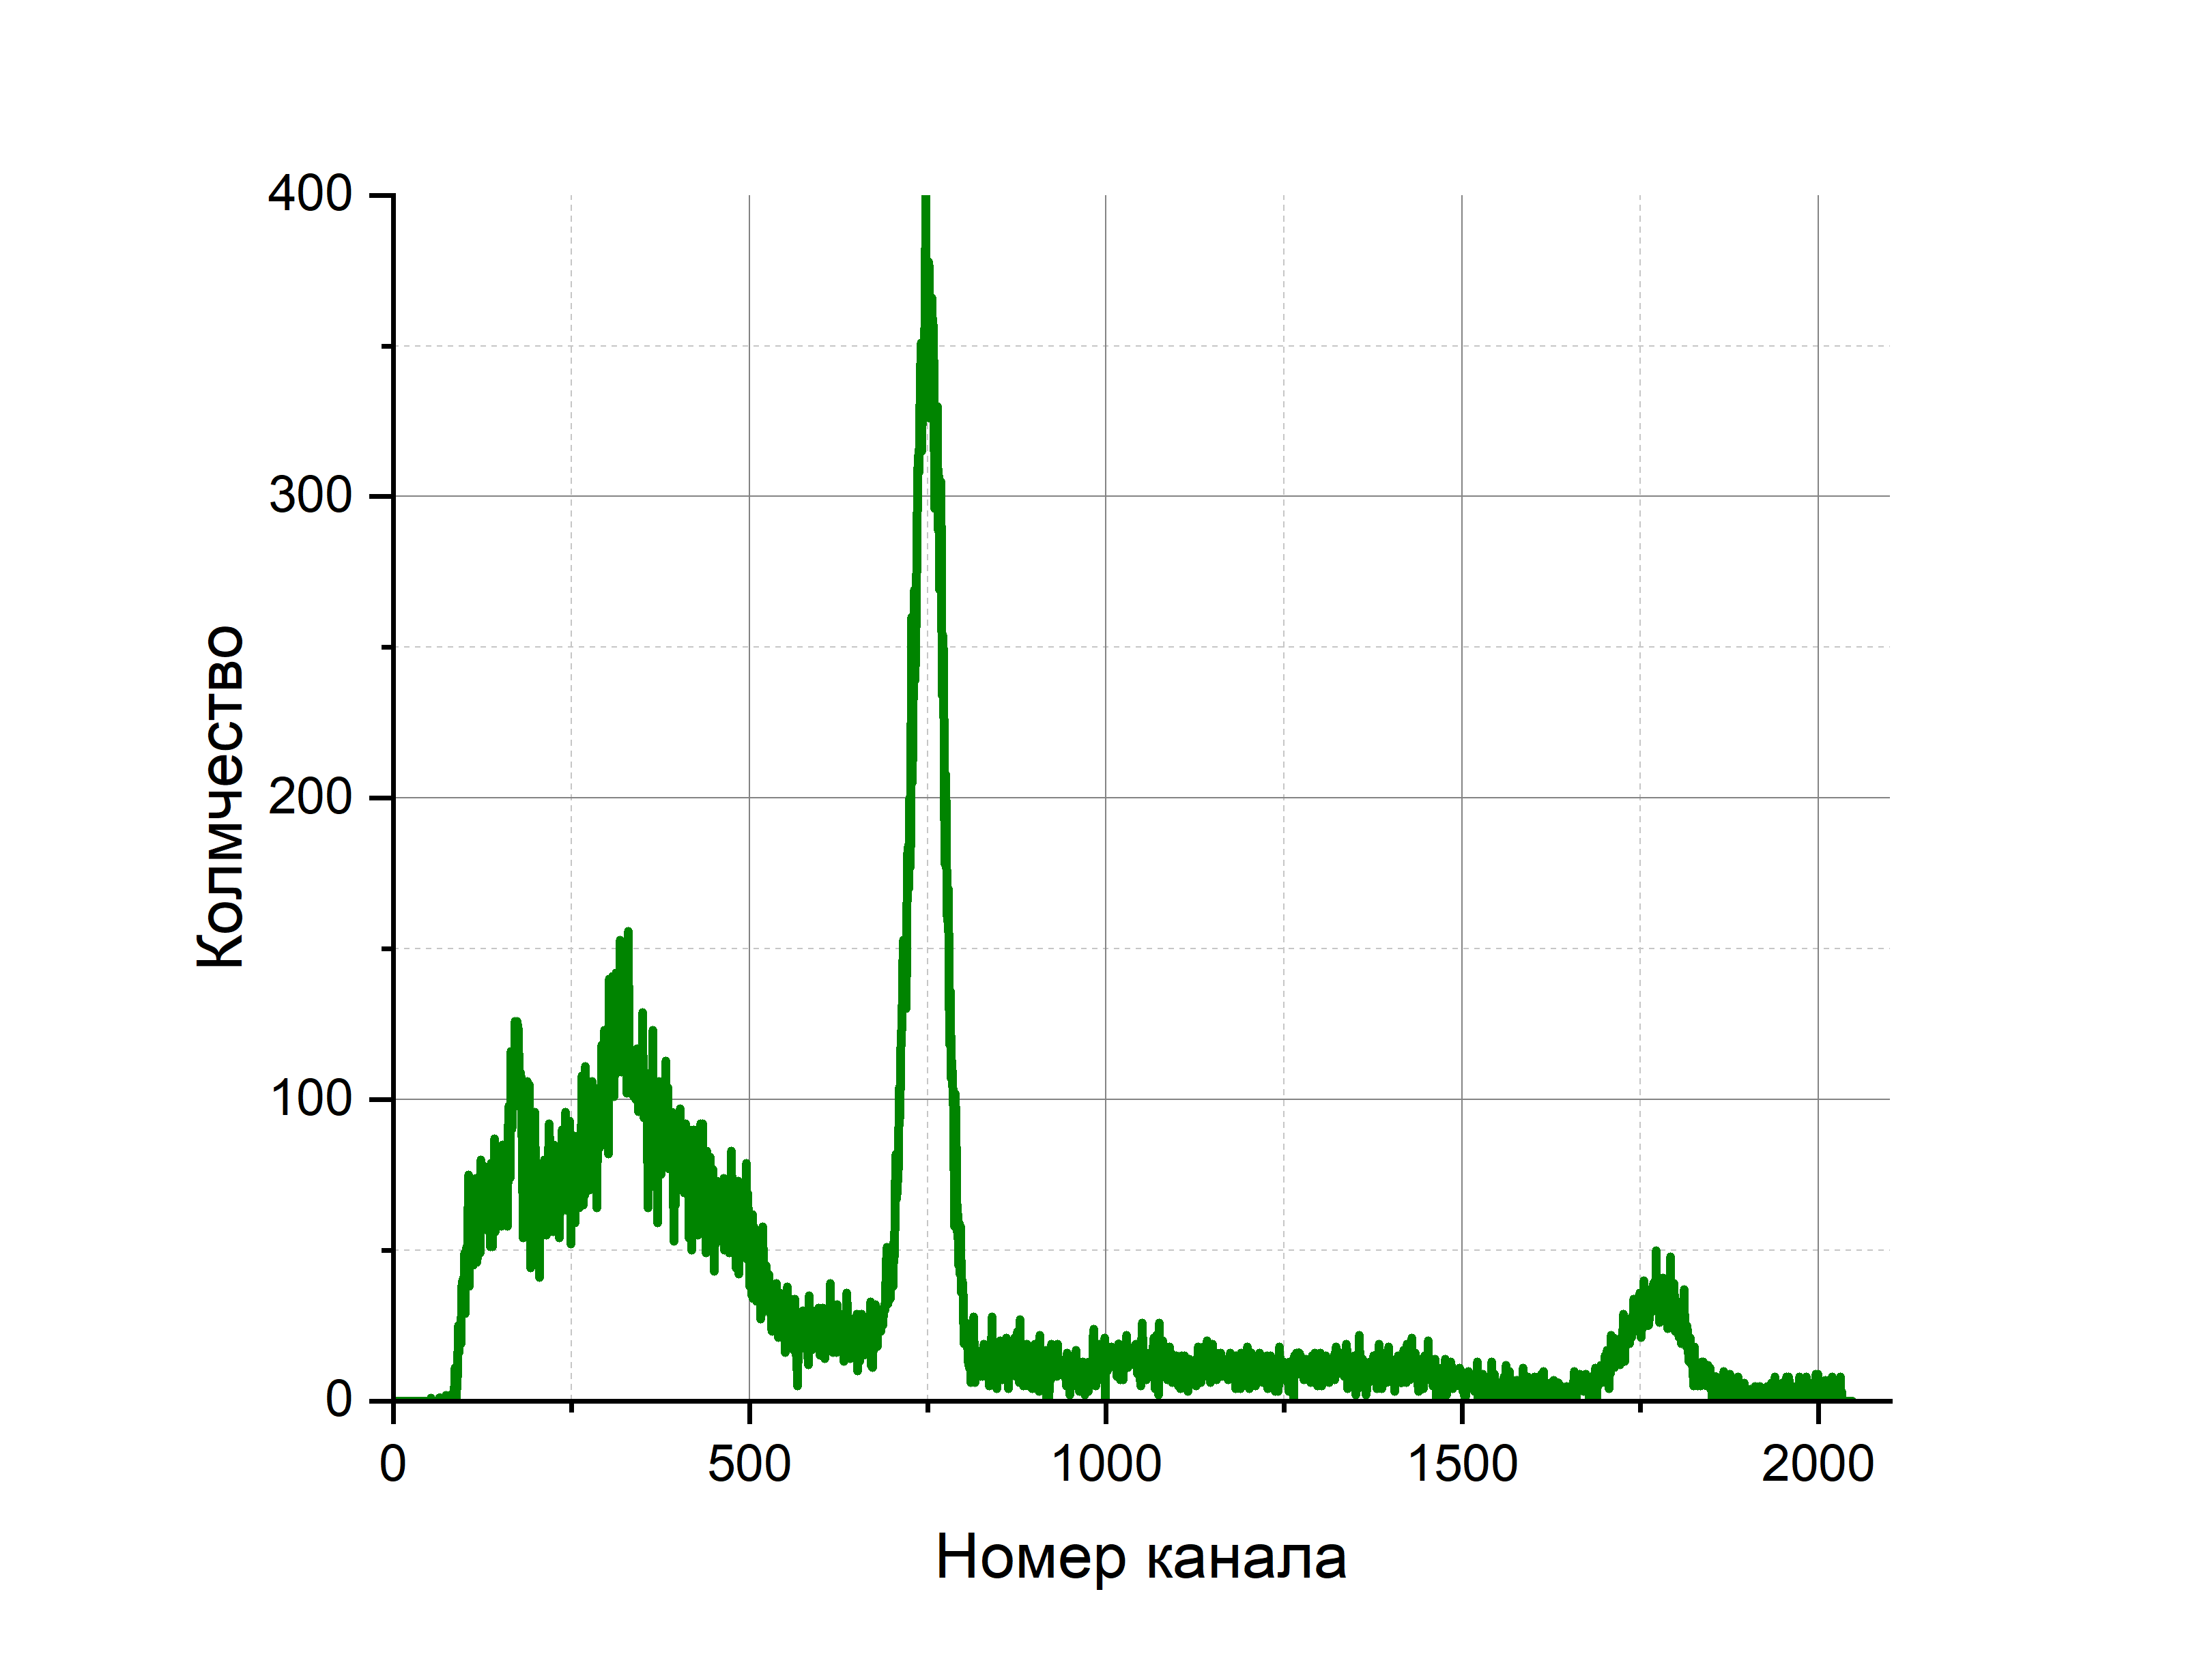
\includegraphics[width=0.8\linewidth]{graph7}
	\caption{Спектр для $^{22}Na$}
	\label{graph6:Na}
\end{figure} 

Зная энергии в спектре $\gamma$-излучения $^{60}Co$ ($1,17$ МэВ, $1,33$ МэВ)  и в спектре $^{137}Cs$ ($0,662$ МэВ), построим калибровочный график $N(E)$ для пересчета номера канала в энергию

\begin{figure}[h!]
	\centering
	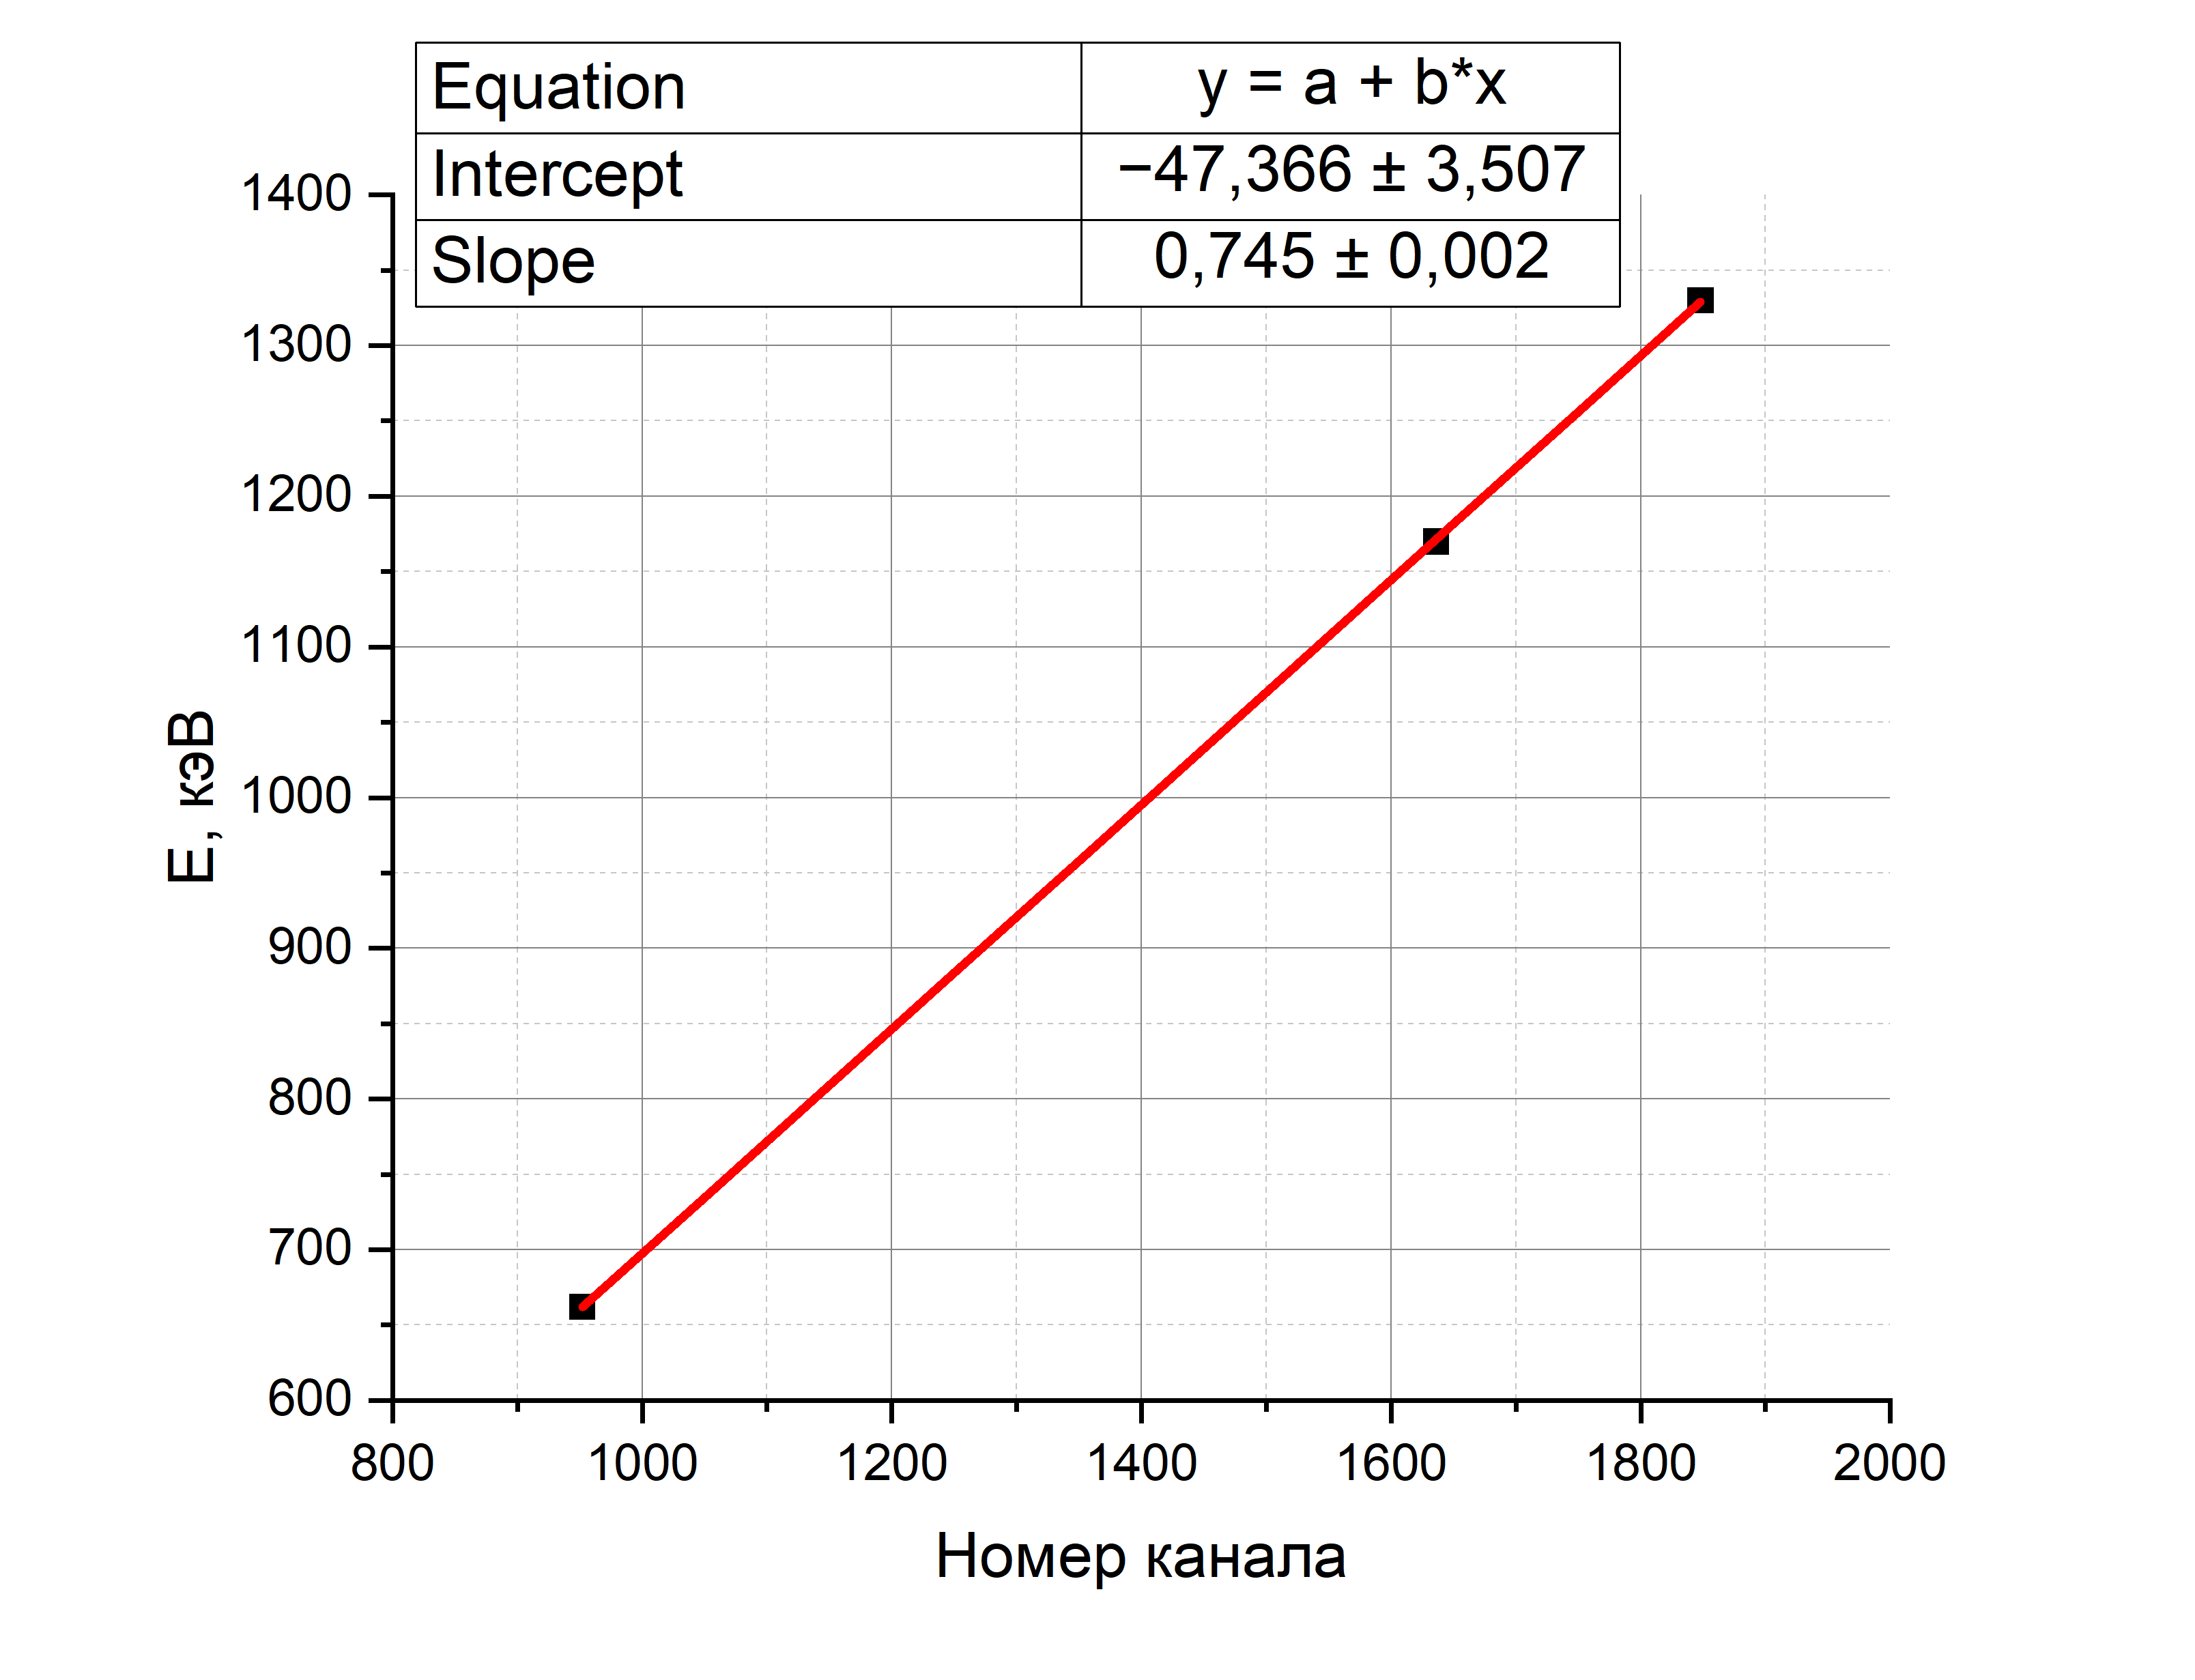
\includegraphics[width=0.8\linewidth]{graph1}
	\caption{Калибровочный график $N(E)$ для пересчета номера канала в энергию}
	\label{graph7:calibration}
\end{figure}
 
Получили, что $b = (0,745 \pm 0,002)$ кэВ, $a = (-47,366 \pm 3,507)$ кэВ.

\newpage
 
Используя данный график, определим для всех образцов значения энергий пиков полного поглощения $E$, их ширину на половине высоты $\Delta E$ и энергетическое разрешение $R$. Данные занесем в Таблицу %ref{table1:}
 
По полученным данным, построим график зависимости $R^2 = f(1/E)$.

\begin{figure}[h!]
	\centering
	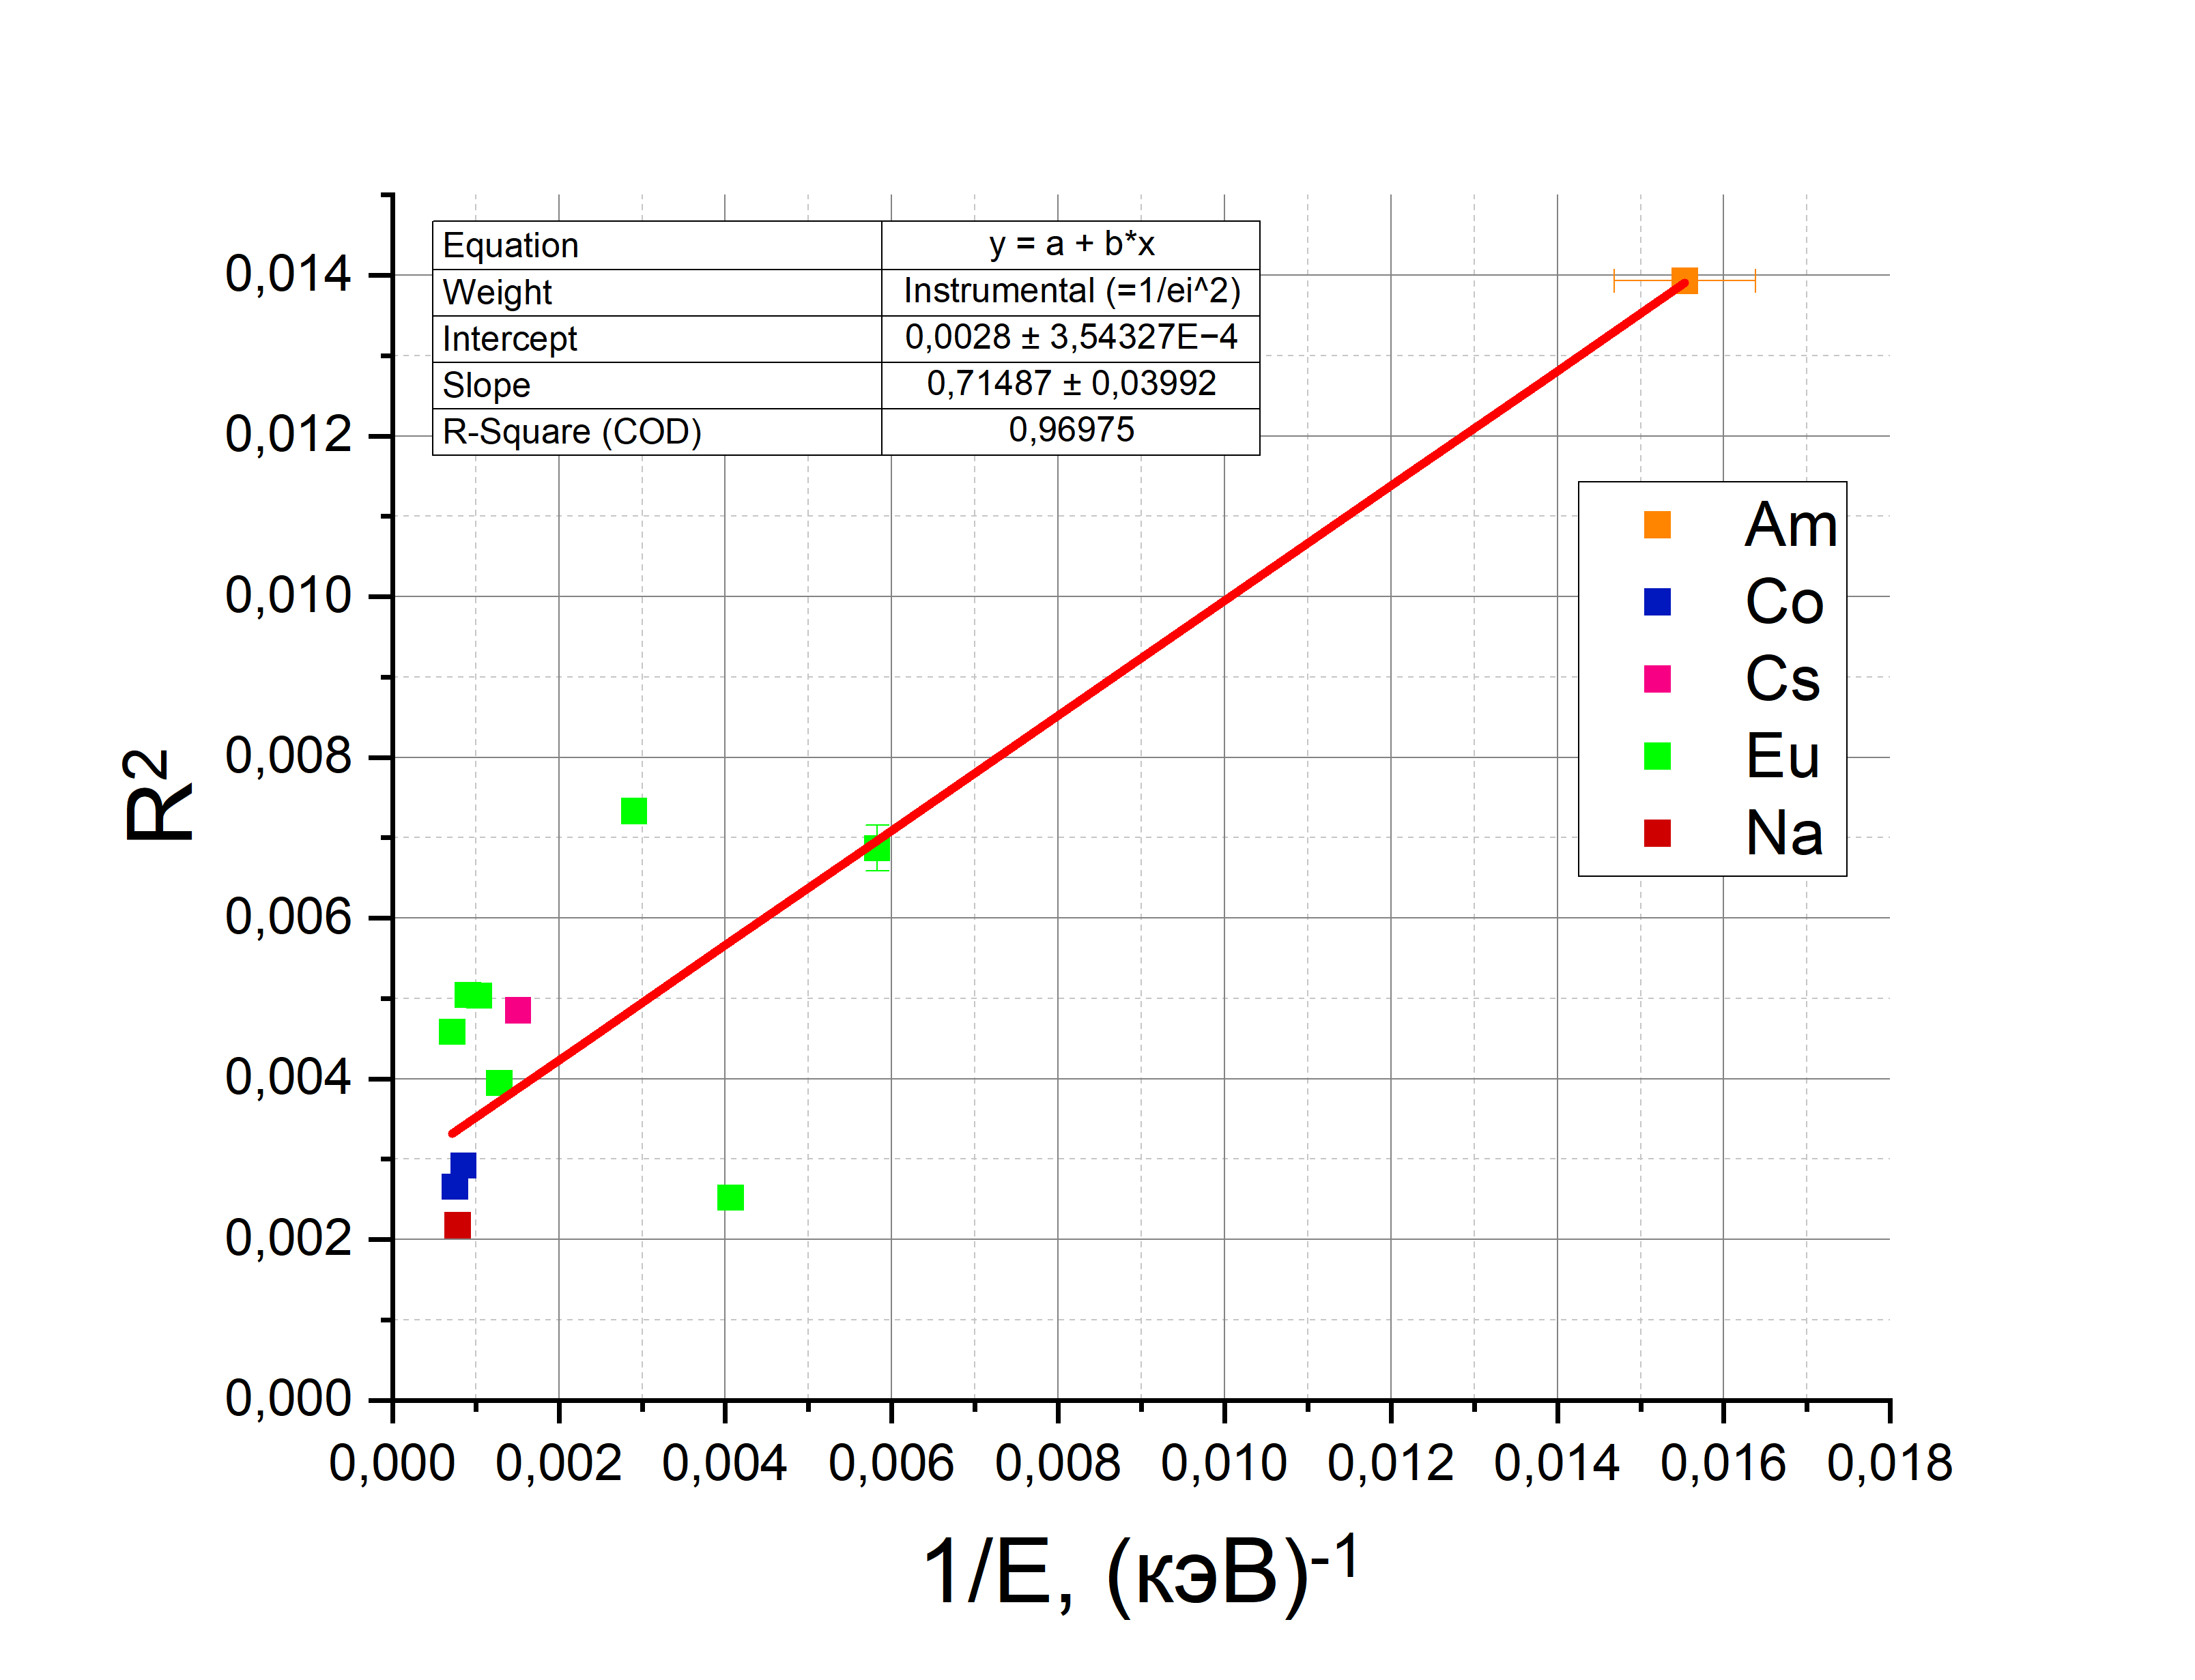
\includegraphics[width=0.8\linewidth]{graph2}
	\caption{Зависимость квадрата энергетического разрешения от величины, обратной к энергии $R^2 = f(1/E)$}
	\label{graph8:R^2}
\end{figure}

Где погрешности рассчитывались согласно формулам:

\begin{align*}
	\sigma^2_{\frac{1}{E}} &= \frac{N^2 \sigma^2_b + \sigma^2_a}{E^2} \\
	\sigma^2_{R^2} &= 4R^2 \left( \frac{N^2 \sigma^2_b}{E^2} + \frac{\Delta E^2}{E^4} (N^2 \sigma^2_b + \sigma^2_a) \right) \\
\end{align*}

\newpage

\subsubsection*{Обратное рассеяние}

Для $^{60}Co$, $^{22}Na$, $^{137}Cs$, из спектров удается определить энергию обратно рассеянных электронов. Построим график зависимости энергии пика обратного рассеяния от энергии фотопика:

\begin{figure}[h!]
	\centering
	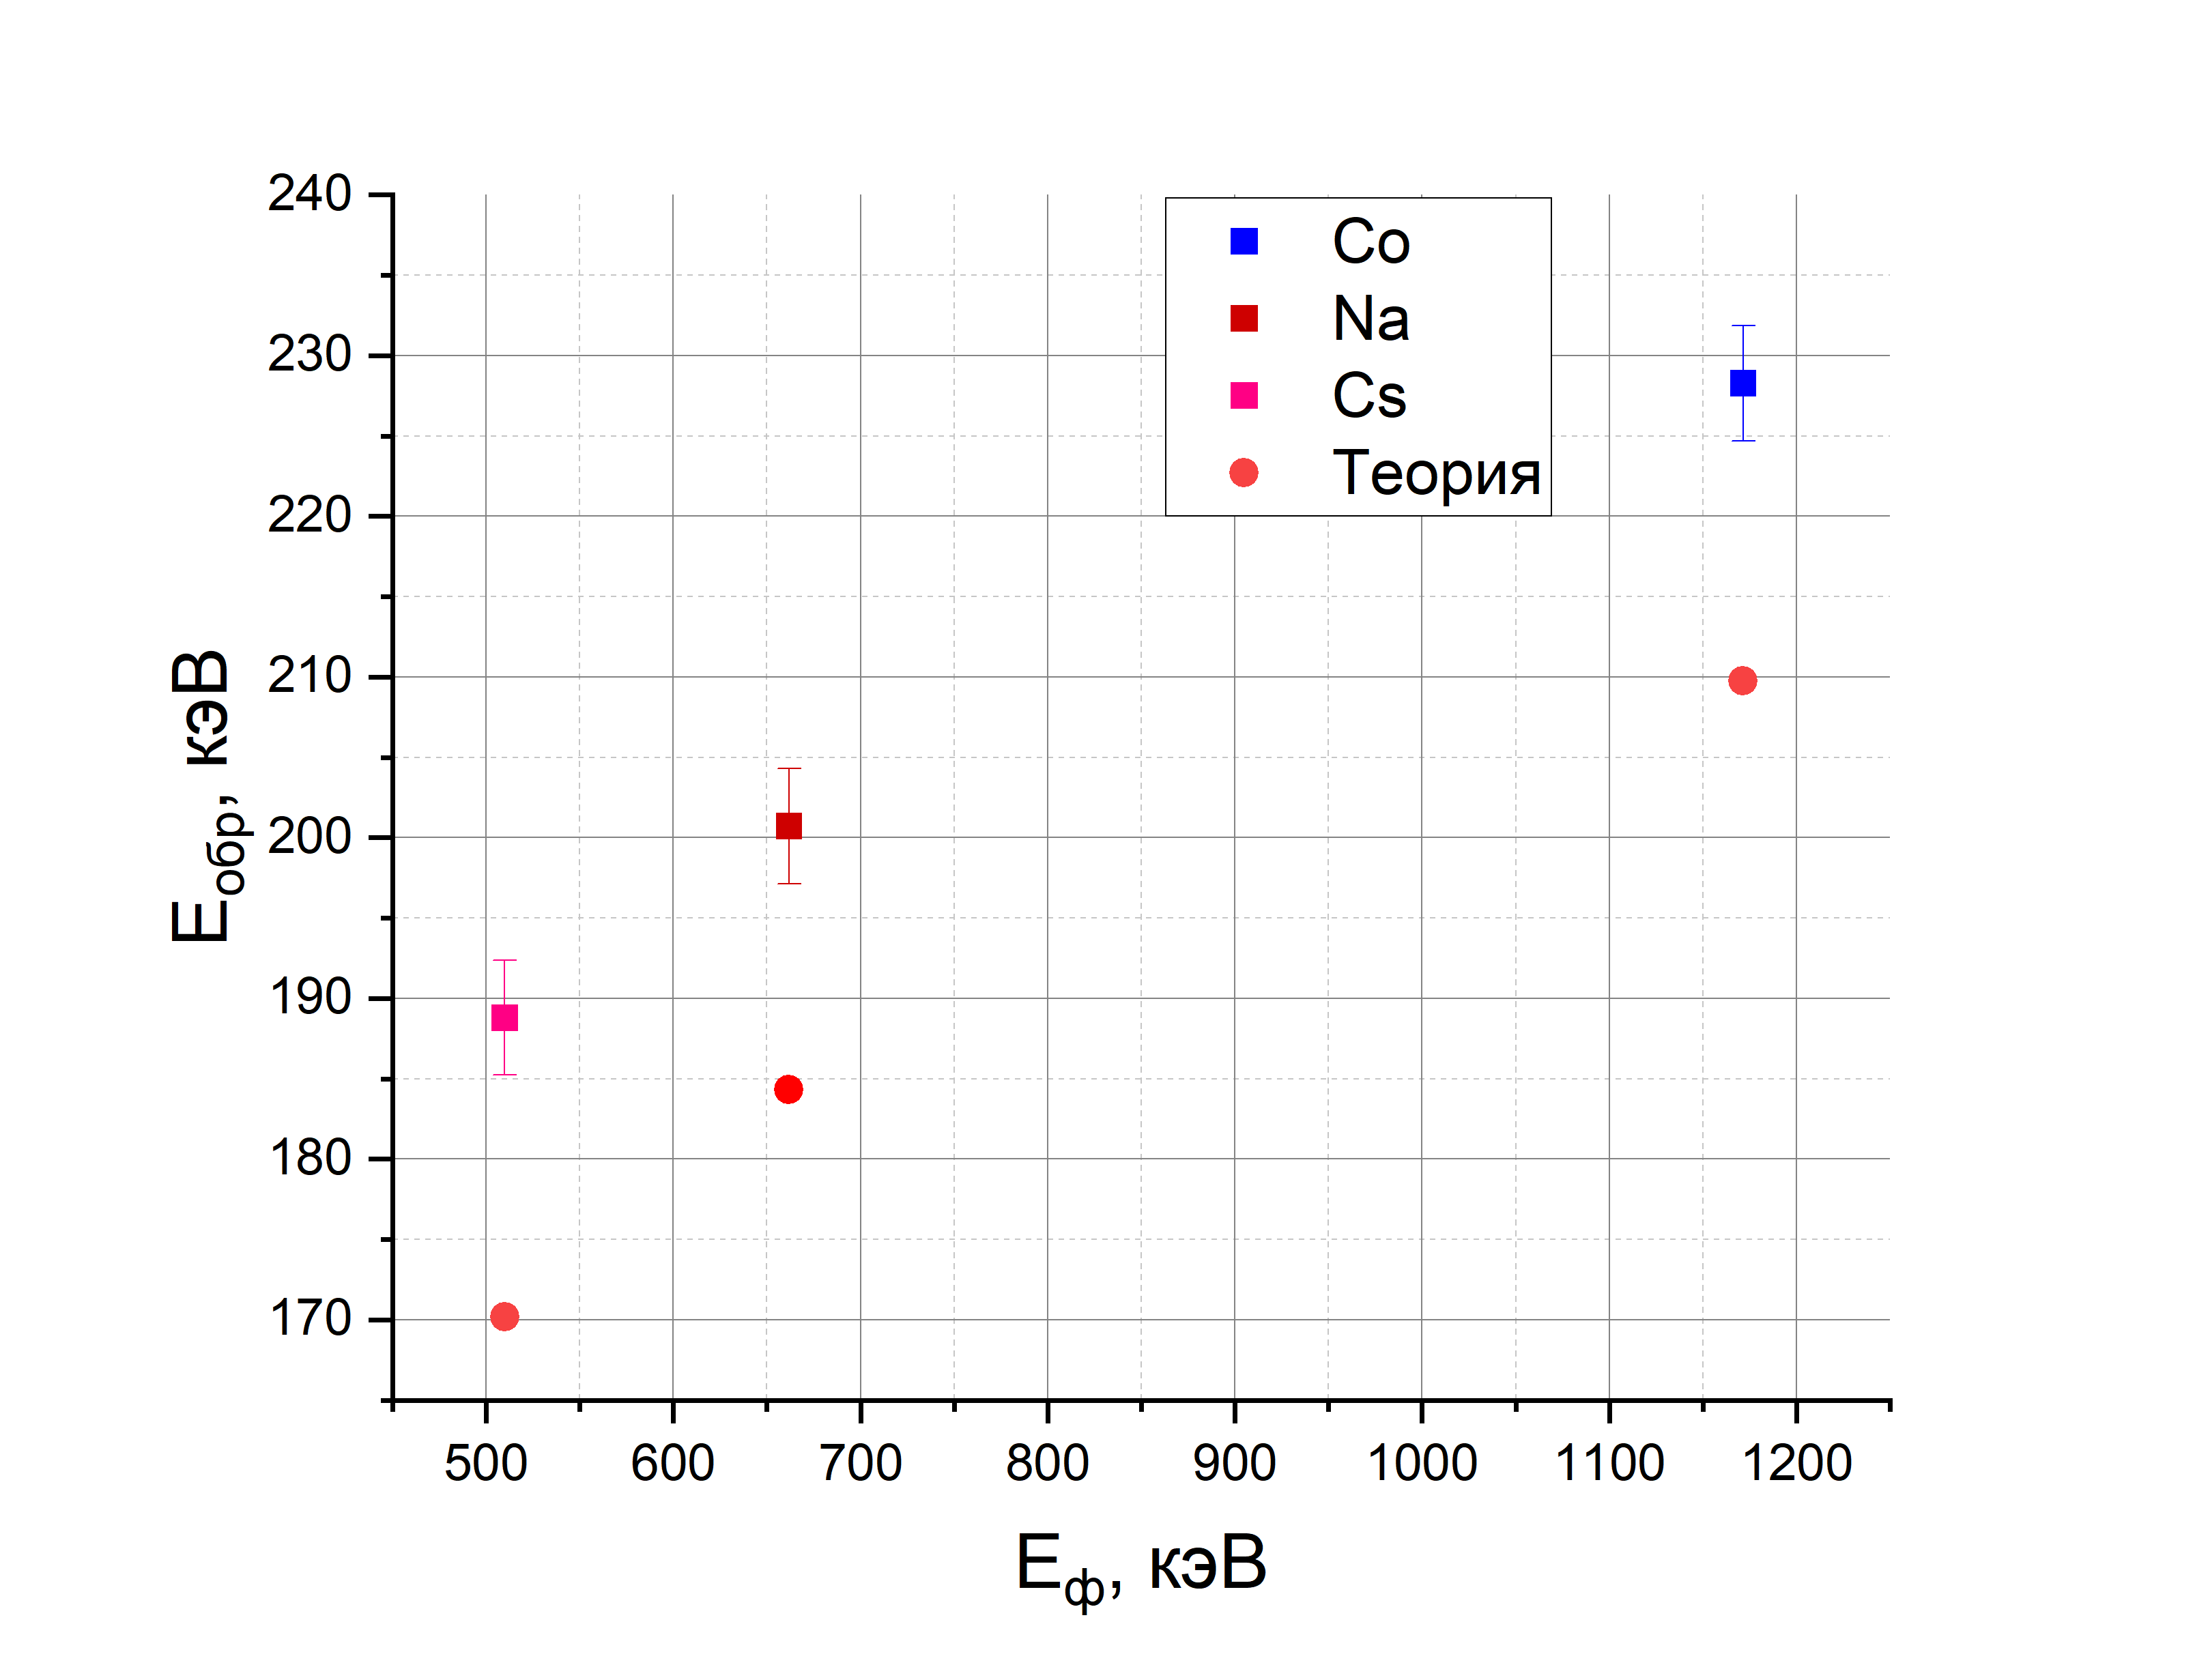
\includegraphics[width=0.8\linewidth]{graph9}
	\caption{Зависимости энергии пика обратного рассеяния от энергии фотопика: теоретическая и экспериментальная}
	\label{graph9:Back}
\end{figure}

\subsubsection*{Комптоновское рассеяние}

Только в спектрах $^{60}Co$ и $^{137}Cs$ удалось различить край комптоновского поглощения. Сравним их с теоретическими значениями

Для $^{60}Co$:

\begin{align*}
	E_{experimental} &\approx (980,6 \pm 4,5)  кэВ \\
	E_{theor} &= 963 кэВ
\end{align*}

Для  $^{137}Cs$:

\begin{align*}
	E_{experimental} &\approx (489,0 \pm 3,8)  кэВ \\
	E_{theor} &= 477 кэВ
\end{align*}

\subsubsection*{Внутренняя конверсия}

В спектре $^{137}Cs$ также был замечен узкий пик, энергия которого составляет $E_{experimental} = (30,1 \pm 3,5) кэВ$ -- данный пик может соответствовать явлению внутренней конверсии в атоме цезия. Сравним это значения с табличными данными: $E_{K \alpha} = 30,9 кэВ$. 

Следовательно, данный пик отвечает $K_{\alpha}$ переходу в атоме $^{137}Cs$.
 
\newpage

\subsubsection*{Излучение свинца}

Также, в спектрах образцов можно увидеть пик, соответствующий излучению свинца, служащего защитой спектрометра от внешнего излучения. Рассчитаем данную энергию и сравним с теоретической:

\begin{align*}
	E_{experimantal} &= (77,8 \pm 3,5) кэВ\\
	E_{theor} &= 75 кэВ
\end{align*}

\section*{Выводы} 
 
\begin{itemize}
\item В ходе работы были получены характерные $\gamma$-линии излучения 5 образцов, которые хорошо соотносятся с табличными данными 

\begin{table}[h!]
\centering
\begin{tabular}{|c|c|c|}
\hline
Образец & E, кэВ (Эксперимент) & E, кэВ (Табличные данные) \\ \hline
\multirow{2}{*}{Co} & 1171,45 & 1173,2 \\ \cline{2-3} 
 & 1329,39 & 1332,5 \\ \hline
Cs & 661,87 & 661,7 \\ \hline
\multirow{7}{*}{Eu} & 171,66 & 121,78 \\ \cline{2-3} 
 & 246,16 & 244,7 \\ \cline{2-3} 
 & 344,50 & 344,28 \\ \cline{2-3} 
 & 778,84 & 778,9 \\ \cline{2-3} 
 & 958,38 & 964,1 \\ \cline{2-3} 
 & 1101,42 & 1112,1 \\ \cline{2-3} 
 & 1397,19 & 1408 \\ \hline
Na & 1276,50 & 1274 \\ \hline
Am & 64,38 & 59,54 \\ \hline
\end{tabular}
\end{table}

\item Также были получены характерные значения для края комптоновского поглощения для $^{60}Co$ и $^{137}Cs$.

\item Более того, в спектре $^{137}Cs$ был зарегистрирован узкий пик, который, как выяснилось, отвечает явлению внутренней конверсии

\end{itemize} 
 
\end{document}